\section{\I{The population section}\label{sec:population-section}}

\subsection{Introduction}

The population section\index{Population section} specifies the model of the population dynamics. It describes the model structure, the population partitions and categories, the population processes (e.g., recruitment, ageing, migration, and mortality), the selectivities, and the associated parameters.

The population section includes:

\begin{itemize}
  \item The population structure, the categories and ages in an age-based model;
  \item The initialisation process, the state of the partition at the start of the first year\index{Initialisation}\index{Model ! initialisation};
  \item The years over which the model runs, the start and end years of the model;
  \item The annual cycle, the number of time steps and the processes that are applied in each time step\index{Annual cycle};
  \item The specification of and the parameters for the population processes, processes that add or remove individuals from a partition, or shift individuals between ages and categories in a partition;
  \item The selectivities;
  \item The parameters, their definitions, initial values, prior distributions, and other characteristics; and
  \item Derived quantities, e.g., mature biomass to include in density-dependent processes such as the spawner-recruit relationship
\end{itemize}

\subsection{\I{Population structure}}\label{sub:sec:pop_sec}

The basic structure of the population section of a \CNAME\ model is defined in terms of an annual cycle, time steps, states, and transitions.

The annual cycle defines what processes happen in each model year, and in what sequence. \CNAME\ assumes an annual cycle.

Each year is defined by one or more time steps, with at least one process occurring in each time step. Each time step can represent a specific period of the calendar year, or it can be an abstract sequence of events.

The division of the year into time steps allows the user to specify the exact order in which processes and observations occur throughout the year. The user specifies the time step in which each process occurs. If more than one process occurs in the same time step, the order in which to apply each process is specified in the \command{time\_step} block.

The mortality processes are grouped into a mortality block: in every time step, a mortality block (a group of consecutive mortality-based processes) exists in which individuals are removed from the partition (see Section~\ref{sec:mortality_block}).

The state is the current status of the population at any given time. The state can change one or more times in each time step in each year. The state object must contain sufficient information to determine how the population changes over time, given a model and a complete set of parameters.

The state can undergo a number of possible changes during the annual cycle, called transitions. Transitions are applied by processes. Transitions include recruitment, natural mortality, fishing mortality, ageing, migration, tagging events, and maturation. These transitions are repeated for each year of the model, although some processes can be specified to occur in a subset of years only.

The key element of the state is the partition. The partition separates the total number of individuals in the population into different ages, lengths, and/or categories. The categories include sex, maturity state, area, and species. \CNAME\ has no predefined categories; \emph{all} categories are defined by the user, which differs from CASAL \citep{1388}.

The partitions can be conceptualised as a matrix, where each row represents a category and the columns are the age classes (Figure~\ref{Fig:part}). Each row represents all individuals that category.

The names of categories are user defined. There must be at least one category defined for each model. The model ages are a sequence from $age_{min}$ to $age_{max}$, with the last age optionally a plus group. The age-length relationship for each category must also be defined for an age-based model, although this relationship could be defined as "none". An example of four categories based on sex and area is:

{\small{\begin{verbatim}
	@categories
	format mature.sex
	names        spawn.male   spawn.female   nonspawn.male   nonspawn.female
	age_lengths  male_AL      female_AL      male_AL         female_AL
\end{verbatim}}}

Consider a model of a fish population with a mature fishery and a non-spawning fishery. Assume that the non-spawning fishery occurs in the non-spawning area. The mature fish then migrate to the spawning area, where the spawning fishery occurs. At the end of spawning, these fish, along with the recruits from the previous year, migrate back to the non-spawning area. The fish population can be represented with partitions by age, sex, maturity, and area (spawning and non-spawning areas). So the partition has 8 rows of numbers-at-age, for 2 sexes $\times$ (mature or immature) $\times$ 2 areas.

\begin{figure}[H]
	\centering
	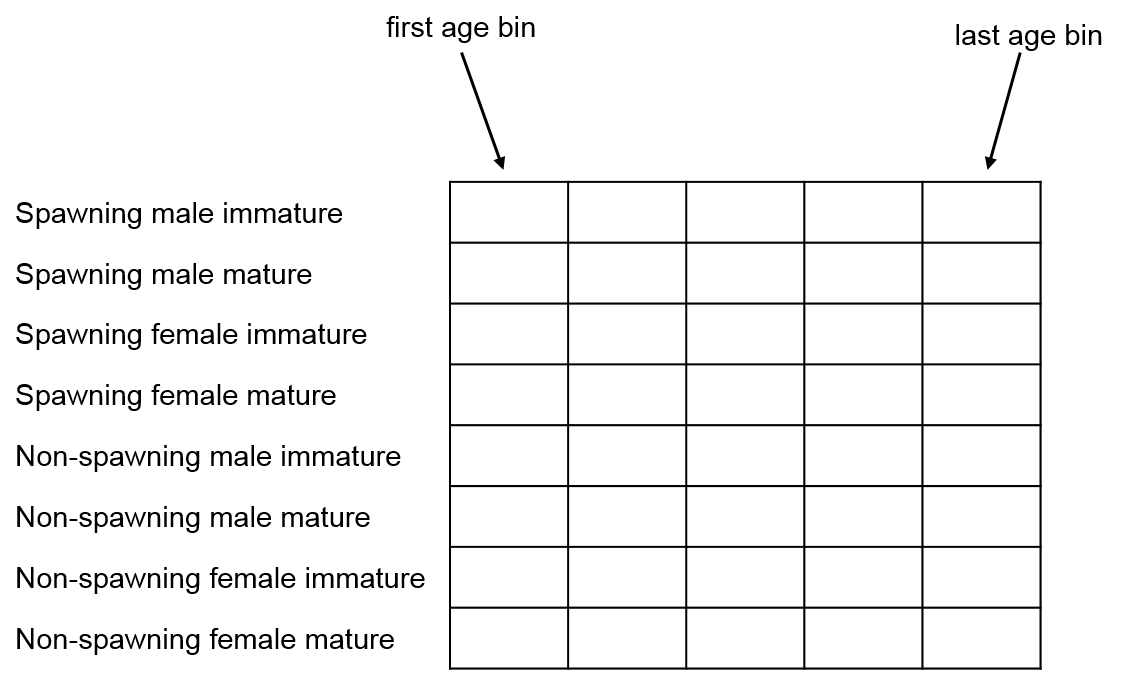
\includegraphics[scale=0.4]{Figures/partition2.png}
		\caption{A visual representation of a partition.}\label{Fig:part}
\end{figure}

For this example four time steps are defined and labelled 1 through 4: \texttt{step1} for the non-spawning fishery period, \texttt{step2} for the migration to the spawning area, \texttt{step3} for the spawning fishery period, and \texttt{step4} for recruitment and migration back to the non-spawning area. The default order of processes within a time step has migrations occurring before fisheries (TODO: check this), so that the processes in steps 2 and 3 could have occurred in one time step. Other details that describe the population structure are also linked to time steps, such as proportion of natural mortality occurring in each time step and in which time step the observations occur.

The definition and ordering of processes in multiple time steps can be used to represent complex dynamics, with the intermingling of multiple species and stocks, migration patterns occurring over multiple areas, and/or multiple sources of anthropogenic impact using a range of methods which cover different areas and times. However, the complexity of a stock structure definition is constrained by the available data. It is challenging to use a complex structure to model a population when there are no observations to support that structure.  For information on how to define categories and use the shorthand syntax see Section~\ref{sec:ShorthandSyntax-section}.

The model is run from the start year through the final year. It can also be run past the final year to project the state of the population through the final projection year.

To specify a model with two categories, male and female, population ages 1-20, with the last age a plus group, three time steps, and sex-specific age-length relationships, the \command{model} and \command{categories} blocks are:

{\small{\begin{verbatim}
		@model
		start_year 1901
		final_year 2000
		projection_final_year 2010
		base_weight_units tonnes
		min_age 1
		max_age 20
		age_plus_group true
		initialisation_phases Equilibrium_phase
		time_steps step1 step2 step3
		
		@categories
		format sex
		names male female
		age_lengths male_growth female_growth
\end{verbatim}}}

\subsection{\I{The state object and the partition}}

The key component of the state object is the partition, a matrix that stores the numbers of individuals at age or length for each category. A category represents a group of individuals that have the same attributes, e.g., life histories characteristics, growth rates, etc.

\begin{itemize}
\item Sex (male or female)
\item Area
\item Maturity (immature or mature)
\item Growth path
\item Tagging event
\item Stock
\item Species
\end{itemize}

A stock is defined as a population of individuals which recruits to that population. Maturity can either be defined as a separate category in the partition, or calculated from the population at the time required; see Section \ref{sec:maturity-notinpartition} for the treatment of maturity when maturity is not a category in the partition.

Each \CNAME\ model requires:

\begin{itemize}
\item The minimum and maximum population ages
\item Whether the maximum age is a plus group
\item The names of all of the categories
\end{itemize}

The age range is sequential by 1 starting with the minimum age through the maximum age.

\CNAME\ allows categories of the partition to exist for a subset of years of a model. This feature enables more efficient computations when models contain categories that do not persist over all model years. A model may define one-off processes that transition individuals from one category into another in a subset of the model initialisation phases or years (e.g., tagging events). Excluding categories for certain years can be more efficient as \CNAME\ will not initialise these categories or apply processes to categories in years or time steps in which they do not exist.

The structure of the partition is defined in a configuration block with the \command{categories} block (Section~\ref{sub:sec:pop_sec}).

Derived quantities are another important component of the state object. An example of a derived quantity is spawning stock biomass (SSB; the biomass of [female] spawning fish calculated at the mid point of the spawning season). \CNAME\ calculates derived quantities using the command \command{derived\_quantity}, which may be required for some processes. In fisheries stock assessment models, a recruitment process which includes a stock-recruitment relationship requires the definition of a derived quantity that specifies the mid-season spawning stock biomass.

\subsection{\I{Time sequences}}

The time sequence of the model is defined in:

\begin{itemize}
  \item \I{The annual cycle}
  \item \I{The mortality blocks}
  \item \I{The initialisation phases}
  \item \I{The model run years}
  \item \I{The projection years}
\end{itemize}

\subsubsection{\I{The annual cycle}}

The annual cycle is implemented as a set of processes that occur in a user-defined order within each year. Time steps are used to break the annual cycle into separate components and allow observations to be associated with specific time periods and processes. Any number of processes can occur within each time step, in any order, although there are restrictions for mortality-based processes (see Section~\ref{sec:mortality_block}); processes can occur multiple times within each time step. Time steps are not implemented during the initialisation phases (effectively there is only one initialisation time step), and the annual cycle in the initialisation phases can be different from the annual cycle specified for the model years.

\subsubsection{\I{The mortality blocks}}\label{sec:mortality_block}

There is an associated \emph{mortality block} for every time step in the annual cycle. Mortality blocks are a key concept in \CNAME.

Mortality blocks are used to define the `point' in the model time sequence when observations (see Section~\ref{sec:observation-section}) are evaluated, and derived quantities (see Section~\ref{sec:derived-quantities}) are evaluated.

A mortality block is defined as a consecutive sequence of mortality processes within a time step. The mortality processes are described in Subsection~\ref{sec:mortality}.

\CNAME\ requires that each time step has exactly one mortality block. Either all of the mortality processes in a time step must be sequential (i.e., there can not be a non-mortality process between any two mortality processes within any one time step); or, if no mortality processes occur in a time step, then the mortality block is defined to occur at the end of the time step.

\CNAME\ will output an error if more than one mortality block occurs in a single time step. Use separate time steps to define a sequence of mortality blocks.

\begin{figure}[H]
	\centering
	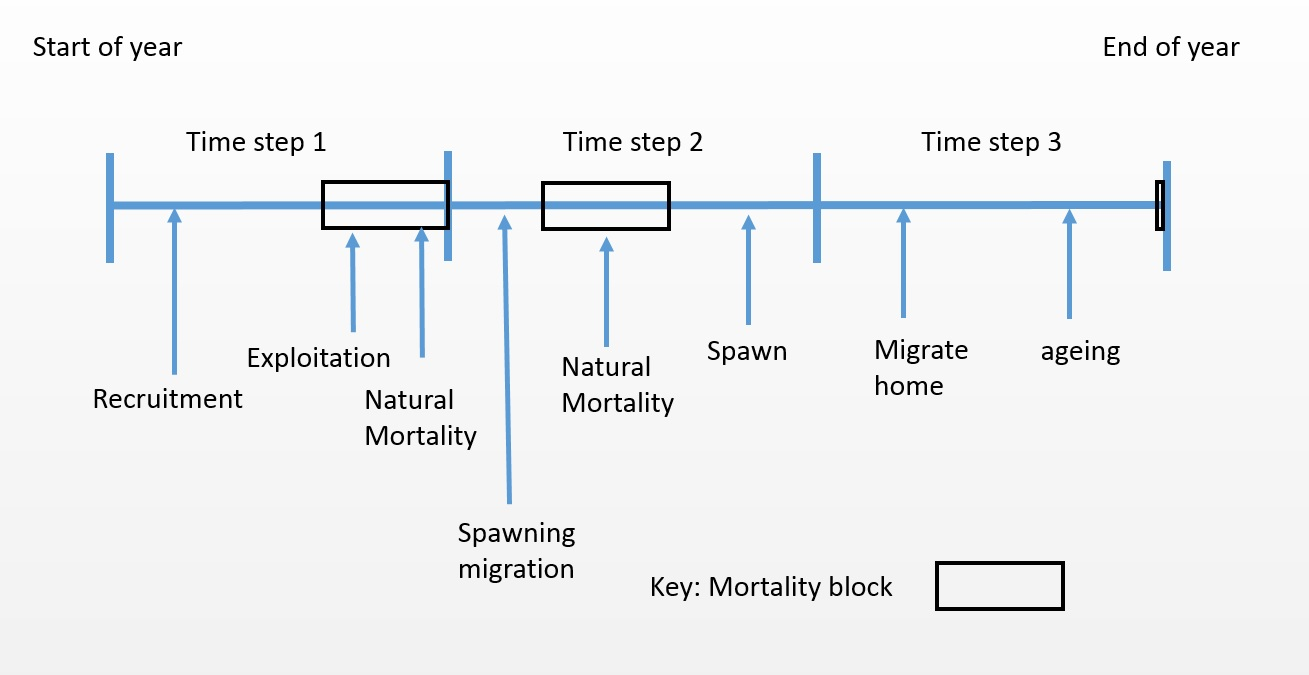
\includegraphics[scale=0.5]{Figures/annual_cycle.jpg}
	\caption{A example sequence for an annual cycle.}\label{Fig:annual}
\end{figure}

\subsubsection{\I{The initialisation phases}}\label{subsec:initialisation}

Initialisation is the process of determining the model starting state. The initial state can be equilibrium/steady state or some other initial state for the model (e.g., exploited), prior to the start year of the model.

There are multiple options for partition initialisation in \CNAME, including

\begin{itemize}
	\item Iterative
	\item Derived
	\item Cinitial
	\item Fixed
\end{itemize}

Model initialisation can also occur in several phases\index{Initialisation!phases}, each of which can use a different method. The initialisations are performed in sequence. At the end of all of the initialisation phases, \CNAME\ then runs through the model years applying the user-defined processes in each time step in the annual cycle.

The multi-phased initialisation allows for flexibility in the number and type of initialisations, for initialising a non-equilibrium starting state, or applying simple processes before applying more complex ones.

Each phase of the initialisation defaults to have the same processes and in the same order as defined in the annual cycle. An initialisation phase can include other processes with the \texttt{insert\_processes} subcommand.

In each initialisation phase, the processes defined for that phase are applied and used as the starting point for the following phase or, if it is the last phase, the start year of the model.

The \emph{first} initialisation phase is always initialised with each age and category set to zero. Care must be taken when using complex category inter-relationships or density-dependent processes that depend on a previously calculated state, as they may fail when used in the first phase of an initialisation.

Multi-phase iterations\index{Multi-phase iteration} can also be used to determine if an initialisation has converged. A second initialisation phase can be added for 1 year, with the same processes applied as in the first phase. The state at the end of the first and second phase is then output. If these states are identical, then it is likely that the initialisation has converged to an equilibrium state.

The subcommands for including or excluding processes are \texttt{insert\_processes} and \texttt{exclude\_processes}.

For the \texttt{insert\_processes} the syntax is:

{\small{\begin{verbatim}
		insert_processes time_step_label(process_label_in_annual_cycle) = label_new_process
\end{verbatim}}}

For example, this subcommand could be used in a \command{time\_step} labelled \texttt{Oct\_Nov}, which includes the \command{process} labelled \texttt{predationInit}, and before the \command{process} labelled \texttt{Instantaneous\_Mortality},

{\small{\begin{verbatim}
		insert_processes Oct_Nov(Instantaneous_Mortality)=predationInit
\end{verbatim}}}

To include a process at the end of the time step:

{\small{\begin{verbatim}
		insert_processes Oct_Nov()=predationInit
		\end{verbatim}}}

To exclude a process from an initialisation phase, use the subcommand \texttt{exclude\_processes} in a command \command{initialisation\_phase},

{\small{\begin{verbatim}
		exclude_processes Instantaneous_Mortality
		\end{verbatim}}}

This command removes the process labelled \texttt{Instantaneous\_Mortality} during that particular initialisation phase.

\paragraph{\I{Iterative Initialisation}}

The \texttt{Iterative} initialisation is a general solution for initialising the model. The iterative method can be slow to converge, depending on the model, but can work on even complex structured models that may be difficult or impossible to implement using analytic approximations.

The number of iterations in the iterative initialisation can increase the model output, and the number of iterations should be chosen to be large enough to allow the population state to fully converge. A period of about two generation times is recommended to ensure convergence. \CNAME\ can be configured to report convergence statistics that can assist in determining convergence properties.

In addition, the iterative initialisation phase can optionally be stopped early if user-defined convergence criteria is met. For a list of supplied years in the initialisation phase, the convergence criteria is met if the proportional absolute summed difference between the state in year $t-1$ and the state in year $t$ ($\widehat{\lambda}$) is less than the user-defined value of $\lambda$, where

\begin{equation}
  \widehat{\lambda} = \frac{\sum\limits_{i} \sum\limits_{j} \left|\text{element}(i,j)_t - \text{element}(i,j)_{t-1} \right|}{\sum\limits_{i} \sum\limits_{j} \frac{}{}\text{element}(i,j)_t}
\end{equation}

Hence, for initialisation define:

\begin{itemize}
  \item The number of initialisation phases,
  \item The number of years in each phase, and
  \item The processes to apply in each phase, where the default processes are those applied in the annual cycle
\end{itemize}

An example with one initialisation phase:

{\small{\begin{verbatim}
@model
...
initialisation_phases Iterative_initialisation

@initialisation_phase Iterative_initialisation
type iterative
years 50
lambda 0.0001
convergence_years 20 40
\end{verbatim}}}

\paragraph{\I{Derived Initialisation}}

The \texttt{Derived} initialisation is an analytical solution that calculates the equilibrium age structure and the plus group using a geometric series solution. The benefit of this method is it can be solved in \texttt{max\_age - min\_age + 1} years/steps/units?, so it is computationally faster than the iterative initialisation phase. Under some process combinations (e.g., one-way migrations) this initialisation does not calculate the exact equilibrium partition. When using this initialisation, confirm that the partition has reached an equilibrium state by either comparing with an iterative initialisation, or by adding a second iterative initialisation phase with a limited number of iterations for comparison.

An example with one initialisation phase:

{\small{\begin{verbatim}
		@model
		...
		initialisation_phases Equilibrium_initialisation

		@initialisation_phase Equilibrium_initialisation
		type derived
		\end{verbatim}}}

\paragraph{\I{Cinitial Initialisation}}

The \texttt{Cinitial} initialisation is used only as a second or greater phase initialisation, and can only be applied after Derived or Iterative initialisation phases. This initialisation can be a method for estimating the non-equilibrium state of population if there is exploitation before the data start. The estimated Cinitial factors shift the initial population away from an equilibrium state prior to the start year. It would be helpful to include an observation of age composition data for the first year of the model in order to estimate the non-equilibrium population state.

An example with two initialisation phases:

{\small{\begin{verbatim}
		@model
		...
		initialisation_phases Iterative Cinitial

		@initialisation_phase Iterative
		type iterative
		years 10
		lambda 0.0001
		convergence_years 10 20

		@initialisation_phase Cinitial
		type cinitial
		categories spawn.male+nonspawn.male spawn.female+nonspawn.female
		table n
		spawn.male+nonspawn.male     5e7 5e7 7e6 6e6 5e6 4e6 3e6 2e6 1e6 1e6 1e1 1e1 1e1 1e1
		spawn.female+nonspawn.female 5e7 5e7 7e6 6e6 5e6 4e6 3e6 2e6 1e6 1e6 1e1 1e1 1e1 1e1
		end_table
		\end{verbatim}}}

The Cinitial factors can also be estimated with the syntax

{\small{\begin{verbatim}
	@estimate cinit_male
	parameter initialisation_phase[Cinitial].spawn.male+nonspawn.male
	same initialisation_phase[Cinitial].spawn.female+nonspawn.female
	lower_bound  2e2  2e2  2e2  2e2  2e2  2e2  2e2  2e2  2e2  2e2  2e0  2e0  2e0  2e0
	upper_bound  2e9  2e9  2e9  2e9  2e9  2e9  2e9  2e9  2e9  2e9  2e9  2e9  2e9  2e9
	type uniform
	\end{verbatim}}}

\paragraph{\I{Fixed Initialisation}}

The \texttt{Fixed} initialisation uses a user-defined table as the initial partition numbers-at-age prior to the start year. Models can be initialised by specifying the numbers-at-age for each category. When initialising models with this type, undefined behaviour may be result if the model applies processes that require derived quantities to be calculated in the initialisation phase.

An example with one initialisation phase:

{\small{\begin{verbatim}
		@model
		...
		initialisation_phases Fixed

		@initialisation_phase Fixed
		type state_category_by_age
		categories male female
		min_age 3
		max_age 10
		table n
		male   1000 900 800 700 600 500 400 700
		female 1000 900 800 700 600 500 400 700
		end_table
		\end{verbatim}}}

\subsubsection{\I{Model run years}}

Following initialisation, the model then runs over the user-defined years, from \texttt{start\_year} to \texttt{final\_year}. For this part of the model, the annual cycle can be broken into multiple time steps per year, and observations can be associated with specific time steps.

Processes are applied in the order specified within each time step. These processes can be the same or different from the processes specified for the initialisation phases.

The run years define the years over which the model is to run and the annual cycle within each year. The model runs from the start of year \argument{initial} to the end of year \argument{final}. The projection then extends the run time up to the end of year \argument{project\_final\_year}.

The model properties must be specified:

\begin{itemize}
  \item The number of time steps and the processes applied in each
  \item The first year, the model start year
  \item The last year, the model final year
  \item The last projection year, the model projection final year
\end{itemize}

An example of the syntax:

{\small{\begin{verbatim}
	@model
	start_year 1972
	final_year 2016
	projection_final_year 2021
	## Define the ages in the partition
	min_age 1
	max_age 30
	age_plus true
	base_weight_units tonnes
	initialisation_phases Equilibrium_state
	## Define the annual cycle
	time_steps Sep_Feb Mar_May Jun_Aug

	## Define the "rows" in the partition
	## This is a single sex and area population
	@categories
	format stock
	names HAK4
	age_lengths age_size

	@initialisation_phase Equilibrium_state
	type derived

	## Define the processes in the annual cycle
	## A list of labels in each time step that correspond to a process
	@time_step Sep_Feb
	processes Recruitment Instantaneous_Mortality

	@time_step Mar_May
	processes Instantaneous_Mortality

	@time_step Jun_Aug
	processes  Ageing Instantaneous_Mortality
\end{verbatim}}}


\subsubsection{\I{Projection years}}\label{sec:projection}

The Projection functionality runs the model forwards, using stochastic and/or deterministic values for some population parameters, such as recruitments and catches.

The \CNAME\ command to run the model in projection mode is \texttt{casal2 -f 1}. The number that follows the \texttt{-f} parameter indicates the number of projections to generate for each set of parameters supplied. This functionality allows for the exploration of many scenarios with a single set of parameters. The number of projections should be greater than 1 only if applying a projection type that is stochastic.

The \texttt{-{}-tabular} flag should be used when running projections after a Bayesian analysis. This option will output a tabular report (see Section~\ref{sub:tabular}) which can then be analysed in \R.

Projection years are after the model run years, and are defined as the \subcommand{final\_year + 1} through the \subcommand{final\_projection\_year}.

For a projection run in \CNAME\, the model is initialised and run through the model years from \argument{start\_year} to \argument{final\_year}. During this run mode \CNAME\ stores all parameter values so that projection classes can allow parameters before \subcommand{final\_year} to be projected. The model then is re-run from \argument{start\_year} to \argument{projection\_final\_year}, where any parameter can either be fixed or drawn from a stochastic distribution or process.

An example of when a parameter is projected before the projection phase has started is for year class parameters. The last few year class parameters may be poorly estimated, which depends on the quality and coverage of the composition data that could inform these parameters or the use of a recruitment index. Thus, users may assume that these parameters are unknown and apply projection methods for the future values.

\CNAME\ has no default projection properties for parameters that are specified by year, e.g., year class strength parameters. The projections for these parameters must be specified using the \command{project} command block. \CNAME\ will produce errors if run in projection mode without a \command{project} block for the \subcommand{ycs\_values} parameter being specified.

\CNAME\ allows any estimable parameter to be specified in a \command{project} block and then used in a projection. The available projection types for these parameters include:

\begin{itemize}
	\item constant
	\item lognormal
	\item empirical-lognormal
	\item empirical re-sampling
	\item user-defined
\end{itemize}

The projection classes available, and examples of their syntax, are in  Section~\ref{sec:projections}.

The subcommands \subcommand{years} and \subcommand{parameter} are common to all projection methods. The argument \argument{multiplier} is a constant which is multiplied with the projected value after it has been generated.

\textbf{Note for the year class parameters:} the definition of year applies to the \argument{ycs\_years}, not the model years. As defined in Section~\ref{subsubsec:BH-recruitment}, \argument{ycs\_years} are offset between the time of spawning and when individuals are added to the partition.

\subsection{\I{Population processes}}

Population processes are processes that change the model state. These processes produce changes in the partition by adding and removing individuals, or by moving individuals between ages and/or categories.

The population processes include:

\begin{itemize}
\item recruitment\index{Recruitment},
\item ageing\index{Ageing},
\item growth\index{Growth},
\item maturation\index{Maturation},
\item mortality\index{Mortality} events (e.g., natural and fishing), and
\item category transition processes\index{Category transition}, i.e., processes that move individuals between categories while preserving their age structure.
\end{itemize}

There are two types of processes: (1) processes that occur across multiple time steps in the annual cycle, e.g., \subcommand{mortality\_constant\_rate} and \subcommand{mortality\_instantaneous}; and (2) processes that occur only within the time step in which they are defined. These processes are applied in the user-defined order when initialising the model, and then for a user-defined order in each year in the annual cycle\index{Annual cycle}.

\subsubsection{\I{Recruitment}}

Recruitment processes are defined as processes that add new individuals to the partition. \CNAME\ has three options for recruitment processes, constant recruitment\index{Recruitment ! Constant}, \I{Beverton-Holt recruitment}\index{Recruitment ! Beverton-Holt} \citep{1203}, and  \I{Beverton-Holt recruitment with deviations}\index{Recruitment ! Beverton-Holt}.

In the recruitment processes, a number of individuals are added to a single age class within the partition, with the number determined by the type of recruitment process specified. If more than one category (of recruits?) is defined, then the proportion of recruits to be added to each category is specified by the \argument{proportions} property, or multiple recruitment processes can be defined. For example, if recruiting to categories labelled \texttt{male} and \texttt{female}, then the proportions may be set to $0.5$ and $0.5$, so that half of the recruits are added to the male category and the other half to the female category.

Recruitment can differ between a spawning event or the creation of a cohort/year class. In a fisheries context, recruitment usually refers to individuals "recruiting" to a fishery. This definition is used because there is usually not a lot of information on younger age classes between the time of spawning and being vulnerable to a survey or fishery for data collection. Thus, the model configuration may specify the population for which data are available.

The offset between spawning and recruitment is parameterised either by the recruitment variable \texttt{age}, or \texttt{min\_age}, which is the default value for the \texttt{age} property in the recruitment process. The \CNAME\ parameter \texttt{age} is the same as the CASAL parameter \texttt{y\_enter}.

For the constant and Beverton-Holt recruitment processes, the  number of individuals following recruitment in year $y$ is

\begin{equation}
N_{y,a,j} \leftarrow N_{y,a - 1,j} + p_j(R_y)
\end{equation}

where $N_{y,a,j}$ is the numbers in year $y$ and category $j$ at age $a$, $p_j$ is the proportion added to category $j$, and $R_y$ is the total number of recruits in year $y$.

\paragraph{\I{Constant recruitment}}\label{subsubsec:constant-recruitment}

In the constant recruitment process the total number of recruits added in each year $y$ in age $a$ is $R_y$, with $R_y = R_0$ for all years

\begin{equation}
  R_{y,j} = p_j(R_0)
\end{equation}

Constant recruitment is equivalent to a Beverton-Holt recruitment process with steepness ($h$) set to 1.

For example, to specify a constant recruitment process where individuals are added to the male and female immature categories at $age=1$ in equal proportion (\texttt{proportions} = 0.5), and the number to add is $R_0=5 \times 10^5$, the syntax is

{\small{\begin{verbatim}
	@process Recruitment
	type constant_recruitment
	categories male.immature female.immature
	proportions 0.5 0.5
	r0 500000
	age 1
\end{verbatim}}}

\paragraph{\I{Beverton-Holt recruitment}}\label{subsubsec:BH-recruitment}

In the Beverton-Holt recruitment process the total number of recruits added each year is $R_y$. $R_y$ is the product of the average recruitment $R_0$, the annual year class strength multiplier $YCS$, and the stock-recruit relationship $SR(SSB_y)$

\begin{equation}\label{eq:BH}
  R_{y,a,j} = p_j(R_0 \times YCS_{ycs\_year} \times SR(SSB_{ycs\_year}))
\end{equation}

where

\begin{equation}\label{eq:year_class}
ycs\_year = y - \texttt{ssb\_offset}
\end{equation}

and $a$ is age, $p_j$ is the proportion of recruits to enter category $j$, and \texttt{ssb\_offset} is the number of years lag between spawning and recruitment.

Recruitment refers to recruitment into the population and may differ from the spawning event. See below on more information about \texttt{ssb\_offset}. In general this parameter should not be specified by the user.

$SR(SSB_y)$ is the Beverton-Holt stock-recruit relationship parametrised by the steepness $h$, and based on \cite{mace_doonan_88} parametrisation

\begin{equation}\label{eq:BH_SR}
SR(SSB_y) = \frac{SSB_y}{B_0} / \left( 1-\frac{5h-1}{4h} \left( 1-\frac{SSB_y}{B_0} \right) \right)
\end{equation}

The Beverton-Holt recruitment process requires a value for \Bzero\ and $SSB_y$ to calculate the number of recruits. A derived quantity (see Section \ref{sec:derived-quantities}) must be defined that provides the annual $SSB_y$ for the recruitment process. \Bzero\ is then defined as the value of the $SSB$ at the end of one of the initialisation phases, which is defined by the parameter \texttt{b0\_initialisation\_phase}.

During initialisation the $YCS$ multipliers are assumed to be equal to 1, and recruitment that happens in the initialisation phases that occur before and during the phase when \Bzero\ is determined are assumed to have steepness $h=1$ (i.e., in those initialisation phases, recruitment is equal to \Rzero).

Recruitment in the initialisation phases after the phase where \Bzero\ was determined are calculated using the Beverton-Holt stock-recruit relationship. \Rzero\ and \Bzero\ have a direct relationship when there are no density-dependent processes in the annual cycle. Models can thus be initialised using \Bzero\ or \Rzero.

The property \texttt{ssb\_offset} should not be manually specified; \CNAME\ determines \texttt{ssb\_offset} by the order of ageing, recruitment, spawning, and the recruitment parameter \texttt{age}

\begin{itemize}
	\item if the annual time step order is recruitment, ageing, spawning, then \texttt{ssb\_offset} should equal \texttt{age} + 1, or
	\item if the annual time step order is spawning, ageing, recruitment, then \texttt{ssb\_offset} should equal \texttt{age} - 1, or
	\item \texttt{ssb\_offset} = \texttt{age}
\end{itemize}

There may be scenarios where the user will input these values, e.g., if there are multiple ageing processes in the annual cycle. \CNAME\ does not have functionality to accommodate this situation, so in this case \texttt{ssb\_offset} would be manually defined.

There are two variants of this process and they refer to how the stock recruitment residuals or $YCS_{ycs\_year}$ are parametrised. This parametrisation can either be in natural space as year class strength ($YCS$) multipliers, or in log space as recruitment deviations. Due to the difference in terminology, these variants are implemented in two separate processes, \subcommand{recruitment\_beverton\_holt} and \subcommand{recruitment\_beverton\_holt\_with\_deviations}, respectively.

\paragraph*{YCS ($YCS_y$)}

The $YCS$ parameter (\texttt{ycs\_years}) is defined in Equation~\eqref{eq:year_class}. The parameter \texttt{ycs\_values} is referenced by the \texttt{ycs\_years} parameter and is important to note when defining \command{estimate}, \command{project}, and \command{time\_varying} blocks for the parameter \texttt{ycs\_values}. An example is at the end of the section.

A common practice when estimating $YCS$ is to standardise using the Haist parametrisation, which was described by V. Haist. \CNAME\ will standardise $YCS$ only if subccommand \subcommand{standardise\_ycs\_years} is defined. The model parameter \texttt{ycs\_values} is a vector \textbf{Y}, covering the years from \texttt{start\_year} - \texttt{ssb\_offset} to \texttt{final\_year} - \texttt{ssb\_offset}, as defined by the parameter \texttt{ycs\_years}. The resulting year class strengths are calculated by $YCS_i=Y_i/\bar{\textbf{Y}}$, where the mean is calculated over the user-specified years \texttt{standardise\_ycs\_years}.

\[
YCS_i =
\begin{cases}
Y_i / mean_{y \in S}(Y_y) & :y \in S\\
Y_i					 & :y \notin S
\end{cases}
\]

where S is the set of years from \texttt{standardise\_ycs\_years}. One effect of this parametrisation is that \Rzero\ is then defined as the mean estimated recruitment over the set of years $S$, because the mean $YCS$ multiplier over these years will always be one.

Typically \texttt{standardise\_ycs\_years} is defined to span the years over which $YCS$ is reasonably well estimated. For years that are not well estimated, $Y_y$ can be set to 1 for some or all years $y\in S$ (which is equivalent to forcing $R_y$ = \Rzero\ x $SR(SSB_y)$) by setting the lower and upper bounds of these $Y$ values to 1. An exception to this might occur for the most recent $YCS$ values, which the user may estimate but not include in the definition of \Rzero\ (because the estimates may be based on too few data). One or more years may be excluded from the range of years for the averaging process of the Haist parametrisation.

The advantage of the Haist parametrisation is that a large penalty is not necessary to force the mean of the $YCS$ parameter to be 1, although a small penalty should still be used to stop the mean of \textbf{Y} from drifting. These adjustments may improve MCMC performance. Projected $YCS$ values are not affected by this feature. A disadvantage with this parametrisation in a Bayesian analysis is that the prior applies to $Y$, not $YCS$.

An example of the specification of a Beverton-Holt recruitment process, where individuals are added to the category "immature" at $age=1$, and the number added is $R_0=5 \times 10^5$; \texttt{SSB\_derived\_quantity} is a derived quantity that specifies the total spawning stock biomass that contributed to the year class, with \Bzero\ the value of the derived quantity at the end of the initialisation phase labelled \texttt{phase1}; and $YCS$ are standardised to have mean one in the period 1995 to 2004, and recruits enter into the model two years following spawning

{\small{\begin{verbatim}
	@process Recruitment
	type recruitment_beverton_holt
	categories immature
	proportions 1.0
	r0 500000
	b0_initialisation_phase phase1
	steepness 0.75
	age 1
	ssb SSB_derived_quantity
	standardise_ycs_years 1995:2004
	ycs_years   1994   1995   1996   1997   1998   1999   2000   2001   2002   2003   2004   2005   2006
	ycs_values  0.65   0.87    1.6   1.13 1.0235  0.385  2.653   1.35      1      1      1      1      1
\end{verbatim}}}


\paragraph*{Recruitment deviations, $\epsilon_y$}

Recruitment deviations represent the stock-recruitment relationship residuals in log space, with the link between $YCS_y$ and $\epsilon_y$

\begin{equation}\label{eq:recruit_devs}
	YCS_y = exp(\epsilon_y - b_y\sigma^2_R / 2)
\end{equation}

where $\epsilon_y\sim N(0,\sigma^2_R)$, $\sigma^2_R$ is the variance of the stock-recruitment residuals, and $b_y$ is a bias correction defined by \cite{methot2011adjusting}

\begin{equation}\label{eq::bias}
b_y = \left\{\begin{array}{lr}
0, & \text{for }y\leq y_1^b\\
b_{max}(1 - \frac{y - y_1^b}{y_2^b - y_1^b}), & \text{for } y_1^b < y < y_2^b\\
b_{max}, & \text{for } y_2^b\leq y \leq y_3^b\\
b_{max}(1 - \frac{y_3^b - y}{y_4^b - y_3^b}), & \text{for }  y_3^b< y < y_4^b\\
0, & \text{for } y_4^b\leq y
\end{array}\right\}
\end{equation}

The $\epsilon_y$ values are normally distributed in log space and thus lognormal when back-transformed to the resulting stock-recruitment relationship $YCS_y$. Recent work has found that this transformation does not technically lead to the \textit{a priori} assumption that the resulting $YCS_y$ are lognormal. See appendix~\ref{investigating-two-options-for-ycs-prior-distribution-formulations} for more discussion.

The ramp function described above for the bias correction has the additional subcommands controlling the ramp as follows,

\begin{itemize}
	\item $y_1^b = $ \subcommand{last\_year\_with\_no\_bias}
	\item $y_2^b = $ \subcommand{first\_year\_with\_bias}
	\item $y_3^b = $ \subcommand{last\_year\_with\_bias}
	\item $y_4^b = $ \subcommand{first\_recent\_year\_with\_no\_bias}
	\item $b_{max} = $ \subcommand{b\_max}
\end{itemize}

{\small{\begin{verbatim}
		@process Recruitment
		type recruitment_beverton_holt_with_deviations
		categories immature
		proportions 1.0
		r0 500000
		last_year_with_no_bias 1940
		first_year_with_bias 1950
		last_year_with_bias 2016
		first_recent_year_with_no_bias 2018
		b_max 0.85
		b0_initialisation_phase phase1
		steepness 0.75
		age 1
		ssb SSB_derived_quantity
		deviation_years   1994   1995   1996   1997   1998   1999   2000   2001   2002   2003   2004   2005   2006
		deviation_values  0 -0.2 0.4 0 0 0 0 0 0 0 0 0 0
\end{verbatim}}}


To specify a Beverton-Holt recruitment for each stock, the information required is:

\begin{enumerate}
	\item $YCS$, starting from year (\texttt{start\_year} - \texttt{ssb\_offset}) and extending up to year (\texttt{final\_year} - \texttt{ssb\_offset})
	\item the value of \texttt{age} (a.k.a. \texttt{y\_enter} to CASAL users)
	\item the steepness parameter \texttt{h}
	\item in a multi category model, the proportion of recruits for each category
	\item a label for the derived quantity
\end{enumerate}

Also note when an \command{initialisation\_phase} (Section~\ref{subsec:initialisation}) type = \subcommand{derived} is specified and the recruitment is defined by \subcommand{b0}, then all categories must be specified in the \command{recruitment} block. Usually in a recruitment processes you only need to define the categories that receive recruits. Say, for example, a population had a spawning area different from the area that recruits enter the population, then an area specific model could be specified containing spawning categories and recruiting categories. recruiting categories would be specified in the subcommand \subcommand{categories}, as these will be the categories receiving recruits. \textbf{If} you have \command{initialisation\_phase}, \subcommand{type=derived} you need also to specify all categories that are a part of that recruitment process, e.g.,

{\small{\begin{verbatim}
		@process Recruitment
		type recruitment_beverton_holt
		categories recruits.male recruits.female spawn.male spawn.female
		proportions 0.5 0.5 0.0 0.0
		r0 500000
		ssb SSB
		....
		\end{verbatim}}}
The proportions = 0.0 are needed due to the way the derived initialisation phase works, i.e., it finds a solution for when \subcommand{r0} = 1.0 based on an infinite geometric series for the plus group, and scales the initial partition by \subcommand{r0}. Thus, if all categories are not specified, then those that are missed would not be initialised to true values and this could lead to inaccurate model outputs. This caution extends to multiple-stock fisheries models where all the categories that make up the stock need to be listed.
\subsubsection{\I{Ageing}\label{sec:ageing}}

The ageing process `ages' individuals --- simply, moving all individuals in the named categories $j$ from one age class $a$ to the next $a + 1$, or accumulates them if the last age class is a plus group.

The ageing process is defined as,
\begin{equation}
  \text{element}(a,j) \leftarrow \text{element}(a + 1,j)
\end{equation}

except in the case of the plus group (if defined),
\begin{equation}
  \text{element}(a_{\text{max}}, j) \leftarrow \text{element}(a_{\text{max}}, j) + \text{element}(a_{\text{max}-1}, j).
\end{equation}

For example, to apply ageing to the categories \texttt{immature} and \texttt{mature}, then the syntax is,

{\small{\begin{verbatim}
	@process Ageing
	type ageing
	categories immature mature
	\end{verbatim}}}

\textbf{Note} that ageing is \emph{not} applied by \CNAME\ by default. As with other processes, \CNAME\ will not apply a process unless it is defined and specified as a process within the annual cycle. Hence, it is possible to specify a model where a category is not aged. \emph{\CNAME\ will not check or otherwise warn if there is a category defined where ageing is not applied.}

\subsubsection{\I{Mortality}\label{sec:mortality}}

Eight types of mortality processes are permissible in \CNAME: constant rate, event, biomass-event, instantaneous, instantaneous retained, Hollings, initialisation, and a density-dependent relationship based on prey suitability. These processes remove individuals from the partition, either as a rate, as a total number (abundance), as a biomass of individuals or as a mixture of these. Note that \CNAME\ does not (yet) implement the Baranov catch equation. However, instantaneous mortality is considered an approximation to the Baranov catch equation. To apply both natural and biomass-event mortality \texttt{mortality\_instantaneous} can be specified. Note that all mortality processes occur within a mortality block of a time step see Section~\ref{sec:mortality_block} for more information and definitions on mortality blocks.

\paragraph{Constant mortality rate}
To specify a constant annual mortality rate \index{Constant mortality}(e.g. $M=0.2$) for categories `male' and `female', then,
{\small{\begin{verbatim}
@process NaturalMortality
type mortality_constant_rate
categories male female
selectivities One One
m 0.2 0.2

\end{verbatim}}}

\begin{equation}
D_{j,t} = \sum_a N_{a,j} (1 - \exp{S_{a,j} M_j p_t})
\end{equation}
Where, $D_{j,t}$ is the number of deaths in category $j$ in time step $t$, $N_{a,j}$ is the number of individuals in category $j$ at age $a$. $S_{a,j}$ is the selectivity value for age $a$ in category $j$, $M_j$ is the mortality rate for category $j$, and $p_t$ is the proportion of the mortality rate to apply in time step $t$.

Note that the mortality rate process requires a selectivity. To apply the same mortality rate over all age classes, use a selectivity defined as $S_j=1.0$ for all ages $j$, e.g.,

{\small{\begin{verbatim}
@selectivity One
type constant
c 1
\end{verbatim}}}

You can also apply age specific mortality rates. For example consider the hypothesis that mortality is higher for younger and older individuals and lowest when individuals are at their optimal fitness. This could be done using a double exponential selectivity (see Section~\ref{sec:selectivities} for what that selectivity looks like);

{\small{\begin{verbatim}
@selectivity age_specific_M
type double_exponential
x0 7.06524
x1 1
x2 17
y0 0.182154
y1 1.43768
y2 1.57169
alpha 1.0

@process NaturalMortalityByAge
type mortality_constant_rate
categories male female
selectivities age_specific_M age_specific_M
m 1.0 1.0
\end{verbatim}}}

In the above syntax you can see how you set \subcommand{m} to zero and allow the rate to be described through the selectivity. This concept can be applied in other mortality methods such as \subcommand{instantaneous\_mortality}.
\paragraph{Event and biomass-event mortality}

The event mortality\index{Event mortality} and biomass-event mortality\index{Biomass-event mortality} processes act in a similar manner, except that they remove a specified abundance (number of individuals) or biomass respectively. These can be used to include anthropogenic mortality where numbers of removals are known, e.g. fishing in a fisheries model, rather than applying mortality as a rate.

In these cases, the abundance or biomass removed is also constrained by a maximum exploitation rate. \CNAME\ removes as many individuals, or as much biomass, as it can while not exceeding the maximum exploitation rate. When minimising, event mortality processes require a penalty to discourage parameter values that will not allow the defined number of individuals to be removed. Here, the model penalises those parameter estimates that result in an too low a number of individuals in the defined categories (after applying selectivities) to allow for removals at the maximum exploitation rate (and similarly for biomass). See Section \ref{sec:penalties} for more information on how to specify penalties.

For example, the event mortality applied to user-defined categories $i$, with the numbers removed at age $j$ determined by a selectivity-at-age $S_j$ is applied as follows:

First, calculate the vulnerable abundance for each category $j$ in $1 \ldots J$ for ages $a = 1 \ldots A$ that are subject to event mortality,
\begin{equation}
  V(a,j) = S(a) N(a,j)
\end{equation}

and, hence, define the total vulnerable abundance $V_{total}$ as,
\begin{equation}
  V_{total}  = \sum\limits_j {\sum\limits_a {V(a,j)}}
\end{equation}

Hence the exploitation rate\index{Maximum exploitation rate} to apply is
\begin{equation}
U = \begin{cases}
  C/V_{total}, & \text{if $C/V_{total} \leq U_{max}$} \\
  U_{max}, & \text{otherwise}\\
  \end{cases}
\end{equation}

And the number removed $R$ from each age $a$ in category $j$ is,
\begin{equation}
  R(a,j) = UV(a,j)
\end{equation}

For example, to specify an \textbf{abundance based} fishing mortality process in a fisheries model, with catches given for a set of specific years, over categories `immature' and 'mature', with selectivity `FishingSel', and assuming a maximum possible exploitation rate of 0.7, the syntax is,

{\small{\begin{verbatim}
	@process Fishing
	type event_mortality
	categories immature mature
	years 2000 2001 2002 2003
	U_max 0.70
	selectivities FishingSel FishingSel
	penalty event_mortality_penalty
	\end{verbatim}}}

and specifed similarly for a \textbf{biomass} based fishing mortality process,

{\small{\begin{verbatim}
		@process Fishing
		type mortality_event_biomass
		categories immature mature
		years 2000 2001 2002 2003
		U_max 0.70
		selectivities FishingSel FishingSel
		penalty event_mortality_penalty
		\end{verbatim}}}

\paragraph{Instantaneous mortality}\label{subsubsec:instantaneous-mortality}

The instantaneous mortality process\index{Instantaneous mortality} combines both natural mortality and event biomass mortality into a single process. This allows the simultaneous application of both natural mortality and anthropogenic mortality to occur across multiple time steps. This process applies half the natural mortality in each time step, then the mortalities from all the concurrent removals instantaneously, then the remaining half of the natural mortality. In fisheries models this is the most commonly used mortality process. It allows for multiple removal events in the case of a fisheries model multiple fisheries/fleets. There are a few constraints that a removal method can only occur in one time step, but you can have multiple removals to cover events during the year.

When instantaneous mortality is applied the following equations are used.

\begin{itemize}
	\item An exploitation rate (actually a proportion) is calculated for each fishery, as the catch divided by the selected-and-retained biomass,
	$$ U_f = \frac{C_f}{\sum_a \bar{w}_aS_{f,a}n_a e^{-0.5tM_a}}$$
	\item The mortality pressure associated with method $f$ is defined as the maximum proportion of fish taken from any element of the partition in the area affected by the method $f$,
	$$ U_{f,obs} = max_a(\sum_k S_{k,a}U_k) $$
	where the maximum is over all partition elements affected by fishery $f$, and the summation is over all methods $k$ which affect the jth partition element in the same time step as fishery $f$.

In most cases the mortality pressure will be equal to the exploitation rate (i.e., $U_{f,obs} = U_f$), but can be different if: (a) there is another removal method operating in the same time step as removal method $f$ and affecting some of the same partition elements, and/or (b) the selectivity $S_{f,a}$ does not have a maximum value of 1.

There is a maximum mortality pressure limit of $U_{f,max}$ for each method of removal $f$. So, no more than proportion $U_{f,max}$ can be taken from any element of the partition affected by removal method $f$ in that time step. Clearly, $0 \leq U_{max} \leq 1$. It is an error if two removal methods, which affect the same partition elements in the same time step, do not have the same $U_max$.

For each $f$, if $U_{f,obs} > U_{f,max}$, then $U_f$ is multiplied by $U_{f,max}/U_{f,obs}$ and the mortality pressures are recalculated. In this case the catch actually taken from the population in the model will differ from the specified catch, $C_f$.

\item The partition is updated using
	$$ n'_a = n_a exp(-tM_a)\big[1 - \sum_f S_{f,a} U_f \big] $$
\end{itemize}

As an example, to apply natural mortality of $0.20$ across three time steps on both male and female categories, and with two methods of removals (fisheries) \texttt{FishingWest FishingEast} with respective catches (kg) known for years 1975:1977 (the catches are given in the \texttt{catches} table and information on selectivities, penalties and maximum exploitation rates are given in the \texttt{method} table), the syntax is,

{\small{\begin{verbatim}
	@process instant_mort
	type mortality_instantaneous
	m 0.20
	time_step_ratio 0.42 0.25 0.33
	selectivities One
	categories male female
	units kgs

	table catches
	year FishingWest FishingEast
	1975	80000	111000
	1976	152000	336000
	1977	74000	1214000
	end table

	table method
	method       category  selectivity u_max   time_step penalty
	FishingWest   stock     westFSel    0.7     step1     CatchPenalty
	FishingEast   stock     eastFSel    0.7     step1     CatchPenalty
	end_table
	\end{verbatim}}}

and for referencing catch parameters for use in projecting, time\_varying and estimating, the syntax is,
{\small{\begin{verbatim}
		parameter process[mortality_instantaneous].method_"method_label"{2018}
		\end{verbatim}}}
	where \subcommand{"method\_label"} is lower case from the \subcommand{catch} or \subcommand{method} table and continuing the example,

{\small{\begin{verbatim}
		parameter process[instant_mort].method_FishingWest{2018}
		\end{verbatim}}}

If you want weight to be calculated by empirical weight at age matrices as described in Section~\ref{sec:weight-at-age} the method table has an additional column that can call weight at age objects. For example

{\small{\begin{verbatim}
		@age_weight jan_weight_at_age
		type data
		table data
		year 1 		2 		3 		4
		1980 3.4	5.6		7.23 	8.123
		end_table

table method
method       category  selectivity u_max   time_step penalty 		age_weight
FishingWest   stock     westFSel    0.7     step1     CatchPenalty
FishingEast   stock     eastFSel    0.7     step1     CatchPenalty
end_table
\end{verbatim}}}


\paragraph{Instantaneous mortality with retained catch and discards}\label{sec:inst-mort-retained}

The instantaneous mortality retained process\index{Instantaneous mortality retained} builds on the instantaneous mortality process (\ref{subsubsec:instantaneous-mortality}) which has simultaneous applications of fishing and natural
mortality, but with all catch-at-sea being landed, i.e., no discarding. The process \texttt{mortality\_instantaneous\_retained} allows for retained catch, discards, and also a mortality to be applied to discards, i.e., some are allowed to survive. The method for taking catch from the partition and constraints used are the same as in \texttt{mortality\_instantaneous}.

The process was created to solve problems in the pot fishery for blue cod which has a minimum legal size and so some catch must be discarded at sea and some of these discards are expected to survive (based on some experimental work). There are length data taken at sea so that the catch selectivity can be estimated, and length and age data from the landed catch (retained) so that the retention selectivity can also be estimated. In this version of the process, discard mortality is specified by the user by defining a selectivity to represent mortality by age or length (e.g., constant of reverse logistic) and it is intended that it would not be estimated since there is no observation class for it yet. If discard mortality is not provided, it is assumed that all discards die. Landed catch, and both retained and catch selectivites must be specified.

Extending the example shown in instantaneous mortality process (\ref{subsubsec:instantaneous-mortality}) to use retained weight instead of catch, the input commands would be:

{\small{\begin{verbatim}
    @process FishingRetainedCatch
    type mortality_instantaneous_retained
    m 0.20
    #natural mortality
    time_step_ratio 0.42 0.25 0.33 # ratio of natural mortality in each of the tree time steps
    selectivities One
    #for natural mortality by age
    categories male female
    units kgs

    table catches # two fisheries, West and East
    year FishingWest FishingEast
    1975 80000 111000 # these are now landed catch
    1976 152000 336000
    1977 74000 1214000
    end table

    table method #all discards die
    method      category selectivity retained_selectivity u_max time_step penalty
    FishingWest stock    westFSel    westRetainedSel      0.7   step1     CatchPenalty
    FishingEast stock    eastFSel    eastRetainedSel      0.7   step1     CatchPenalty
    end_table
    \end{verbatim}}}

If discard mortality is less than 1.0 is required, then use:

{\small{\begin{verbatim}
    table method # 50% discard mortality
    method      category selectivity retained_selectivity discard_mortality u_max time_step penalty
    FishingWest stock    westFSel    westRetainedSel      DisMort           0.7   step1     CatchPenalty
    FishingEast stock    eastFSel    eastRetainedSel      DisMort           0.7   step1     CatchPenalty
    end_table

    @selectivity DisMort
    Type constant
    c 0.5 #50% mortality of discards returned to the sea
    \end{verbatim}}}

See instantaneous mortality process (\ref{subsubsec:instantaneous-mortality}) for referencing catch parameters and calculating weight using empirical weight by age matrices.

The report gives total catch, actual landed catch, and discards, without and with discard mortality; use the following

{\small{\begin{verbatim}
    @report Mortality
    type process
    process Instantaneous_Mortality_Retained
    \end{verbatim}}}

In the following, fisheries are indexed by $f$, and $a$ indexes both age and category combinations.

The total catch is found using by using a selectivity, $S_{f,a}$, in the same way as in the instantaneous mortality process. Retention, $R_{f,a}$, is defined by specifying a selectivity and it can be a function of length or age. The retained catch is the product of these two values, $R_{f,a} \ S_{f,a}$. If sex is in the partition, then there are potentially two retention curves, one for each sex. In general, there is a retention curve for each category in the partition. It does not apply to surveys. Discard mortality is also specified as a selectivity, $D_{f,a}$. The fraction of dead fish from fishing activity is $S_{f,a} * ( R_{f,a} + (1.0 - R_{f,a} ) * D_{f,a} )$. If $D_{f,a}$ is 1.0, then all selected fish are dead, but if it is 0.0, then only retained fish are dead.

When the \texttt{mortality\_instantaneous\_retained} process is applied, the following equations are used:

\begin{itemize}
    \item Total catch (catch-on-board), $C_{f}$, is calculated by (retained catch) * VF / VR, where VF is vulnerable retained biomass, $j$ indexes categories and $t$ is the proportion of M in the time step, and VF is the full vulnerable biomass, $VF = \sum_{a,j} \overline{w}_{a} S_{a,j} n_{a,j} \exp(-0.5 t M_{a,j})$.

    \item An exploitation rate (actually a proportion) is calculated for each fishery, as the total catch (retained + discards) divided by the selected biomass (VF above) using selectivity $S_{f,a}$,
        $$ U_f = \frac{C_f}{\sum_a \bar{w}_a S_{f,a} n_a \exp(-0.5 t M_{a})}$$

    \item The mortality pressure associated with method $f$ is defined as the maximum proportion of fish taken from any element of the partition in the area affected by the method $f$,
        $$ U_{f,obs} = max_a (\sum_k S_{k,a} U_k) $$
    where the maximum is over all partition elements affected by fishery $f$, and the summation is over all methods $k$ which affect the $j$th partition element in the same time step as fishery $f$.

    In most cases the mortality pressure will be equal to the exploitation rate (i.e., $U_{f,obs} = U_f$), but can be different if: (a) there is another removal method operating in the same time step as removal method $f$ and affecting some of the same partition elements, and/or (b) the selectivity $S_{f,a}$ does not have a maximum value of 1.

    There is a maximum mortality pressure limit of $U_{f,max}$ for each method of removal $f$. So, no more than proportion $U_{f,max}$ can be taken from any element of the partition affected by removal method $f$ in that time step. Clearly, $0 \leq U_{max} \leq 1$. It is an error if two removal methods, which affect the same partition elements in the same time step, do not have the same $U_max$.

    For each $f$, if $U_{f,obs} > U_{f,max}$, then $U_f$ is multiplied by $U_{f,max}/U_{f,obs}$ and the mortality pressures are recalculated. In this case the catch actually taken from the population in the model will differ from the specified catch, $C_f$.

    \item Discard numbers-at-age (including their share of natural mortality) is $S_{a,j} (1 - R_{a,j}) n_{a,j} \exp(-0.5 t M_{a,j})$, and those that die at the end of the time step (updating the partition) are $D_{a,j} S_{a,j} (1 - R_{a,j}) n_{a,j} \exp(-t M_{a,j})$, where $D_{f,a}$ is the fraction that die on return to the sea.

    \item The partition is updated by removing landed catch, natural mortality, and discard mortality
        $$ n'_{a} = n_{a} \exp(-t M_a) \big[ 1 - \sum_f S_{f,a} U_f (R_{f,a} + D_{f,a} (1 - R_{f,a})) \big] $$
\end{itemize}


\paragraph{Holling's mortality rate}

The density-dependent Hollings mortality process\index{Holling mortality} applies the Holling Type II and Type III functions \citep{Holling1959}, but is generalised using the Michaelis-Menten equation \citep{MentenMichaelis1913}. The function removes a number or biomass from a set of categories according to the total (selected) abundance (or biomass) and some 'predator' abundance (or biomass), and constrained by a maximum exploitation rate.

For example, the mortality applied to user-defined categories $k$, with the numbers removed at age $l$, determined by a selectivity-at-age $S(l)$ is applied as follows:

First, calculate the total predator abundance (or biomass) over all predator categories $k$ in $1 \ldots K$ and ages $l = 1 \ldots L$ that are applying the mortality,
\begin{equation}
	P(k,l) = S_{predator}(l) N_{predator}(k,l)
\end{equation}

And define the total predator abundance (or biomass) $P_{total}$ as,
\begin{equation}
	P_{total}  = \sum\limits_K {\sum\limits_L {P(k,l)}}
\end{equation}

Then, calculate the total vulnerable abundance (or biomass) over all prey categories $k$ in $1 \ldots K$ and ages $l = 1 \ldots L$ that are subject to the mortality,
\begin{equation}
	V(k,l) = S_{prey}(l) N_{prey}(k,l)
\end{equation}

And hence, define the total vulnerable abundance (or biomass) $V_{total}$ as,
\begin{equation}
	V_{total}  = \sum\limits_K {\sum\limits_L {V(k,l)}}
\end{equation}

and then, the the number to remove is determined by,
\begin{equation}
	R_{total} = P_{total} \frac{a  V_{total}^{x-1}}{b + V_{total}^{x-1}}
\end{equation}
where $x=2$ for Holling type II function,  $x=3$ for Holling type III function, or any value of $x \geq 1$ for the generalised Michaelis-Menten function, and $a > 0$ and $b > 0$ are the Holling function parameters.

Hence, the exploitation rate\index{Maximum exploitation rate} to apply is,
\begin{equation}
	U = \begin{cases}
		R_{total}/V_{total}, & \text{if $R_{total}/V_{total} \leq U_{max}$} \\
		U_{max}, & \text{otherwise}\\
	\end{cases}
\end{equation}

And the number removed $R$ from each age $l$ in category $k$ is,
\begin{equation}
	R(k,l) = UV(k,l)
\end{equation}

The density-dependent Holling mortality process is applied either as a biomass or an abundance depending on the value of the \texttt{is\_abundance} switch.

For example, a biomass Holling type II mortality process on \texttt{prey} by our predator \texttt{predator} would have syntax,

{\small{\begin{verbatim}
		@process HollingMortality
		type Holling_mortality_rate
		is_abundance F
		a 0.08
		b 10000
		x 2
		categories prey
		selectivities One
		predator_categories predator
		predator_selectivities One
		u_max 0.8
		\end{verbatim}}}

\paragraph{Initialisation-event mortality}

Initialisation event mortality\index{Initialisation event mortality} is a specific process that only can occur in the initialisation phase. It allows users to apply abundance or biomass mortality events specifically in initialisation phases. This can be useful if you wanted to deviate a model from equilibrium before model start. This process applies a single catch for all iterations within the initialisation phase, and mortality will not be applied outside of the initialisation phase. This process should not be embedded in the annual cycle. We advise that this process be used in conjunction with the \texttt{insert\_processes} command in the \command{initialisation\_phase} block. Example syntax to implement such a scenario,

{\small{\begin{verbatim}
initialisation_phases Equilibrium_state Predation_state
time_steps Oct_Nov Dec_Mar

@initialisation_phase Equilibrium_state
type derived

@initialisation_phase Predation_state
type iterative
insert_processes Oct_Nov()=predation_Initialisation

@process predation_Initialisation
type initialisation_mortality_event
categories male.HOKI female.HOKI
catch 90000
selectivities Hakesl Hakesl

time_step Oct_Nov
processes Mg1 Instantaneous_Mortality

@time_step Dec_Mar
processes Recruitment Instantaneous_Mortality
\end{verbatim}}}

Note how the \texttt{initialisation\_mortality\_event} has been specified in the initialisation phase \texttt{Predation\_state} but not in the annual cycle.

\paragraph{Prey-suitability mortality}

The density-dependent prey-suitability process\index{Density-dependent prey-suitability} applies predation mortality from a predator group to its prey groups simultaneously. It removes an abundance (or biomass) from each prey group according to the total (selected) abundance (or biomass) of each prey group, the total (selected) abundance (or biomass) of the other prey groups, some 'predator' abundance (or biomass), and the preference (electivity) of the predator to each prey group, but constrained by a maximum exploitation rate. The predator-prey suitability functions were based on the multispecies Virtual Population Analysis (MSVPA) functions described by \citep{JuradoMolina2005}.

For example, the mortality applied to the user-defined prey group $g$ of category $k$, with the numbers removed at age $l$ determined by a selectivity-at-age $S(l)$ is applied as follows:

First, calculate the total predator abundance (or biomass) over all predator categories $k$ in $1 \ldots K$ and ages $l = 1 \ldots L$ that are applying the mortality,
\begin{equation}
P(k,l) = S_{predator}(l) N_{predator}(k,l)
\end{equation}

And define the total predator abundance (or biomass) $P_{total}$ as,
\begin{equation}
P_{total}  = \sum\limits_K {\sum\limits_L {P(k,l)}}
\end{equation}

Then, given the total vulnerable abundance (or biomass) of prey group $g$ over all categories $k$ in $1 \ldots K$ and ages $l = 1 \ldots L$ that are subject to the mortality,
\begin{equation}
V(g,k,l) = S_{prey}(l) N_{prey}(k,l)
\end{equation}

And define the total vulnerable abundance (or biomass) of each prey group $V(g)_{total}$ as,
\begin{equation}
V(g)_{total}  = \sum\limits_K {\sum\limits_L {V(g,k,l)}}
\end{equation}

And the total availability $A(g)_{total}$ for each prey group as,
\begin{equation}
A(g)_{total} = \frac{V(g)_{total}}{\sum\limits_G {V(i)_{total}}}
\end{equation}

The vulnerable abundance (or biomass) and availability every prey group $g$ in $1 \ldots G$ is calculated simultaneously. Then the abundance (or biomass) to remove from each prey group $g$ is a function of its electivity $E(g)$, the availability of all other prey groups $i$ in $1 \ldots G$, the electivity of the predator for each prey group $E(i)$, and the total consumption rate of the predator $CR$ and its abundance (or biomass) $P_{total}$,
\begin{equation}
R(g)_{total}=P_{total} CR \frac{A(g)_{total} E(g)}{\sum\limits_G {A(i)_{total} E(i)}}
\end{equation}

Hence the exploitation rate\index{Maximum exploitation rate} to apply to each prey group $g$ is
\begin{equation}
U(g) = \begin{cases}
R(g)_{total}/V(g)_{total}, & \text{if $R(g)_{total}/V(g)_{total} \leq U_{max}$} \\
U_{max}, & \text{otherwise}\\
\end{cases}
\end{equation}

And the number removed $R(g)$ in each prey group $g$ from each age $l$ in category $k$ is,
\begin{equation}
R(g,k,l) = U(g)V(g,k,l)
\end{equation}

Note that prey suitability choice occurs only between prey groups specified by the process, and the total predator consumption rate represents the consumption of the predator on those prey groups alone. Also note that the electivities must sum to one. Further, the consumption rate can be modified by a layer, to be cell specific.

The density-dependent prey-suitability process is applied as either a biomass or an abundance depending on the value of the \subcommand{is\_abundance} switch.

Individual categories can be aggregated into prey groups using the '+' symbol. To indicate that two (or more) categories are to be aggregated, separate them with a '+' symbol. For example, to specify two prey groups of two species made up of the males and females in each, then the subcommand would be,

{\small{\begin{verbatim}
		prey_categories maleSpeciesA + femaleSpeciesA maleSpeciesB + femaleSpeciesB
		\end{verbatim}}}

This would indicate that there are two prey groups, \texttt{maleSpeciesA + femaleSpeciesA} and \texttt{maleSpeciesB + femaleSpeciesB}, with each group having its own electivity. For example, a biomass prey-suitability mortality process with an overall consumption rate of $0.8$ of \texttt{species A} and \texttt{species B} (modelled as males and females) by our predator \texttt{predatorSpecies} with electivities between \texttt{species A} and \texttt{species B} of $0.18$ and $0.82$ would have syntax,

{\small{\begin{verbatim}
		@process PreySuitabilityMortality
		type prey-suitability_predation
		is_abundance F
		consumption_rate 0.8
		categories maleSpeciesA + femaleSpeciesA maleSpeciesB + femaleSpeciesB
		electivities 0.18 0.82
		selectivities One One One One
		predator_categories predatorSpecies
		predator_selectivities One
		u_max 0.8
		\end{verbatim}}}

\subsubsection{\I{Transition By Category}}

This process moves individuals between categories. The \CNAME\ partition is user-defined, and this type of process is used to move individuals between categories, and is used to specify processes such as maturation (move individuals from an immature to mature state) or migration (move individuals from one area to another).

\paragraph{Annual transition by category}

A special case is annual transition by category, which allows a transition to occur in a specific subset of years only, where each year can have a different rate.

In both cases, there has to be a one to one relationship between the `from' category and the `to' category, i.e., for every source category there is one target category,

\begin{equation}
	N_{a,j} = N_{a,i} \times P_i \times S_{a,i}
\end{equation}
where $N_{a,j}$ is the number of individuals that have moved to category $j$ from category $i$ in age $a$ and $N_{a,i}$ is the number of individuals in category $i$. $P_i$ is the proportion parameter for category $i$ and $S_{a,i}$ is the selectivity at age $a$ for category $i$.

Note, to merge categories just repeat the `to' category multiple times.

An example, to specify a simple spawning migration of mature males from a western area to an eastern (spawning) area, the syntax is,
{\small{\begin{verbatim}
		@process Spawning_migration
		type transition_category
		from West.males
		to East.males
		selectivities MatureSel
		proportions 1
		\end{verbatim}}}

where \texttt{MatureSel} is a selectivity that describes the proportion of age or length classes that are mature and thus move to the eastern area.

\subsubsection{\I{Tag Release events}}\label{sub:tag_release}
Tagging processes can be age or length based processes, where-by numbers of individuals are moved from an untagged category to a tagged category that the user has defined from the \command{categories} block. Tag release processes can also account for initial tag-induced mortality on individuals. Age-based tag release events take a known number of individuals tagged for each age and do a straightforward category transition, along with extra mortality. Individuals are deducted from the non-tagged categories and shifted into tagged categories. Often, the ages of tagged individuals are not known and length based tagging is the most commonly used tagging process.


Length-based tag release processes are more complicated, as \CNAME\ needs to calculate the age-length matrix and the exploitation by each length-bin to then move the correct numbers-at-age based on the known lengths of release. \CNAME\ also allows for initial tag loss. The algorithm that \CNAME\ follows,


For each length bin ($l$) of the input vector of numbers at length ($\tilde{N_l}$) do the following

$$N_{l,j} = \sum_{a = 1}N_{a,l,j} * S_a$$
where $N_{a,l,j}$ is the numbers at age and length for category $j$ in the partition, and $S_a$ is the selectivity at age $a$.


calculate the total numbers at length ($T_l$) across all source categories at length $l$ taking into account the selectivities

$$T_l = \sum_{j = 1}N_{l,j}$$

Calculate the transition rate for this length bin ($u_l$)

$$u_{l} = \tilde{N_l} / T_l$$



Check that we don't exceed some threshold, usually called a $u_{max}$ which is analagous to the $u_{max}$ in a mortality processes.

\[
u_{l} =
\begin{cases}
u_{max},& \text{if } u_{l} > u_{max} \text{ \textbf{flag a penalty}}\\
u_{l},  & \text{otherwise}
\end{cases}
\]

Calculate the numbers at age in this category that we are going to move by multiplying across the age-length matrix and storing this info by age, for each age we want to accumulated these for all length bins. then move the necessary

$$N_{a,j} += N_{a,l} * u_l$$

The syntax for an example of tag release by length process in \CNAME\ follows,
{\small{\begin{verbatim}
		@process 2005Tags_shelf
		type tag_by_length
		years 2005
		from male.untagged+female.untagged
		to male.2005  female.2005
		selectivities ShelfselMale ShelfselFemale
		penalty tagging_penalty
		initial_mortality 0.1
		table proportions
		year 30 40 50 60 70 80 90 100 110 120 130 140 150 160 170 180 190 200 210 220
		2005  0 0 0.0580 0.1546 0.3380 0.1981 0.1643 0.0531 0.0242 0.0097 0 0 0 0 0 0 0 0 0 0
		end_table
		n 207
		U_max 0.999
		\end{verbatim}}}

The above process will move 207 individuals from a combination of male.untagged and female.untagged categories, based on the combination of growth rates and selectivity into tagged male and tagged female categories based on selectivities and growth rates between.

\subsubsection{\I{Tag Loss}}

Tag Loss is the process which accounts for tags being lost from tagged individual over time due to, for example, tag failure or tags getting knocked off. This process is applied as an instantaneous migration rate that can happen over multiple time steps in the annual cycle. This method assumes that when tags are lost the fish are transferred from the \subcommand{from} category to the \subcommand{to} category. How the tag loss rate is applied depends on whether the fish were only tagged with a single tag (\subcommand{tag\_number\_per\_animal = 1}), double tagged (\subcommand{tag\_number\_per\_animal = 2}) or $n$ tagged (\subcommand{tag\_number\_per\_animal = n}). The syntax for this relationship is,

{\small{\begin{verbatim}
	@process Tag_loss
	type tag_loss
	categories tagged_fish
	tag_loss_rate 0.02
	time_step_ratio 0.25 0.75
	selectivities One
	tag_loss_type single
	year 1985
		\end{verbatim}}}

\subsection{\I{Derived quantities}\label{sec:derived-quantities}}

Some processes require, as arguments, a population value derived from the population state. These are termed \texttt{derived quantities}. Derived quantities are values, calculated by \CNAME\ at the end of a specified time step in every year, and hence have a single value for each year of the model. Derived quantities can be calculated as either an abundance or as a biomass. Abundance derived quantities are simply the count or sum over the categories (after applying a selectivity). Similarly for biomass Biomass derived quantities. Derived quantities are also calculated during the initialisation phases. Therefore, the time step during each phase must also be specified. If the initialisation time steps are not specified, \CNAME\ will calculate the derived quantity during the initialisation phases in every year, at the end of the annual cycle.

Derived quantities are required by some processes, e.g. the Beverton-Holt recruitment process. The Beverton-Holt recruitment process can require an equilibrium biomass ($B_0$) and annual spawning stock biomass values ($SSB_y$) to resolve the stock-recruit relationship. Here, these would be defined as the abundance or biomass of a part of the population at some point in the annual cycle for selected ages and categories, and would be calculated as a derived quantity.

Derived quantities are associated with a mortality block see section~\ref{sec:mortality_block} for more detail on mortality blocks. Users can ask for derived quantities partway through mortality blocks. Currently, two methods are implemented in \CNAME\ to interpolate derived quantities part-way through a mortality block, these are \texttt{weighted\_sum} and \texttt{weighted\_product}, and are defined as,
\begin{itemize}
	\item \texttt{weighted\_sum}: after proportion $p$ of the mortality block, the partition elements are given by $n_{p,j} = (1 - p)n_j + p'_j$

	\item \texttt{weighted\_product}: after proportion $p$ of the mortality block, the partition elements are given by $n_{p,j} = n_j^{1-p} n'^p_j$
\end{itemize}
where, $n_{p,j}$ is the derived quantity at proportion $p$ of the mortality block for category $j$, $n_j$ is the quantity at the beginning of the mortality block and $n'_j$ is the quantity at the end of the mortality block.

As an example, to define a biomass derived quantity (say spawning stock biomass, $SSB$), evaluated at the end of the first time step (labelled \texttt{step\_one}), over all 'mature' male and female categories and halfway through the mortality block using the \texttt{weighted\_sum} method, we would use the syntax,

{\small{\begin{verbatim}
@derived_quantity SSB
type biomass
time_step step_one
categories mature.male mature.female
selectivities One
time_step_proportion 0.5
time_step_proportion_method weighted_sum
\end{verbatim}}}

\subsection{\I{Age-length relationship}\label{sec:age-at-age}}

The age-length relationship defines the length at age (and the weight at length, see Section \ref{sec:mean-weight}) of individuals at age/category within the model. There are three length-age relationships available in \CNAME. The first is the naive no relationship (where each individual has length 1 irrespective of age). The second  and third are the von-Bertalanffy and Schnute relationships respectively. The length-at-age relationship is used to determine the length frequency, given age, and then with the length-weight relationship, a weight-at-age of individuals within an age/category. When defining length-at-age in \CNAME, you must also define a length-weight relationship (see Section \ref{sec:mean-weight} below).The model can incorporate changes in length-at-age during the year —i.e., growth between fish birthdays — by incrementing age as specified by the \subcommand{time\_step\_proportions} parameter.

%\begin{description}
%\item {None:} where the length of each individual is exactly 1 for all ages, in which case the \texttt{none} length-weight relationship must also be used.
\paragraph[None]{\argument{none}}\index{Age-length relationshsip!None}
Where the length of each individual is exactly 1 for all ages, in which case the \texttt{none} length-weight relationship must also be used.

%\item{von Bertalanffy:}\index{von Bertalanffy growth curve} where length at age is defined as,
\paragraph[von Bertalanffy]{\argument{von\_bertalanffy}}\index{Age-length relationshsip!von Bertalanffy}
\begin{equation}
\bar{s}(age)= L_\infty \left( 1 - \exp \left( -k \left(age-t_0 \right) \right) \right)
\end{equation}

%\item{Schnute:}\index{Schnute growth curve} where length at age is defined as,
\paragraph[Schnute]{\argument{schnute}}\index{Schnute}
\begin{equation}
\bar{s}(age)=\displaystyle\begin{cases}
  \left[ y_1^b + (y_2^b - y_1^b) \dfrac{1-\exp \left(-a(age - \tau_1) \right)}{1-\exp \left(-a(\tau_2 - \tau_1) \right)} \right]^{1/b}, & \text{if $a\ne0$ and $b\ne0$} \\
  \AddVspace
  y_1 \exp \left[ \ln \left( y_2 / y_1 \right) \dfrac{1-\exp \left(-a(age - \tau_1) \right)}{1-\exp \left(-a(\tau_2 - \tau_1) \right)} \right], & \text{if $a\ne0$ and $b=0$} \\
  \AddVspace
  \left[ y_1^b + \left( y_2^b - y_1^b \right) \dfrac{age-\tau_1}{\tau_2 - \tau_1} \right]^{1/b}, & \text{if $a=0$ and $b\ne0$} \\
  \AddVspace
  y_1 \exp \left[ \ln \left( y_2/y_1 \right) \dfrac{age-\tau_1}{\tau_2 - \tau_1} \right] , & \text{if $a=0$ and $b=0$} \\
  \end{cases}
\end{equation}
%\end{description}

Note, the von Bertalanffy curve is parameterised by $L_\infty$, $k$, and $t_0$; the Schnute curve \citep{836} by $y_1$ and $y_2$, which are the mean lengths at reference ages $\tau_1$ and $\tau_2$, and $a$ and $b$ (when $b=1$, this reduces to the von Bertalanffy with $k=a$).

\paragraph[Data]{\argument{data}}\index{Age-length relationshsip!Data}
There is an option for users to input empirical length at age by year, this is an alternative to going through a age length growth model such as the von Bertalanffy and Schnute model. \CNAME\ will do a lot of interpolations of missing years for the user and across time steps. There is a condition that the measurements of length at age throughout the model years occur in the same time step.

\subsection{\I{Length-weight relationship}\label{sec:mean-weight}}

There are two length-weight relationships available in \CNAME. The first is the 'naive' --- which the relationship where the weight of an individual, regardless of length, is always 1. The second is the 'basic' relationship, which is the standard cubic function of length.

\paragraph[None]{\argument{none}}\index{Length-weight relationshsip!None}

  \begin{equation}
    \text{mean weight}=1
  \end{equation}

\paragraph[Basic]{\argument{basic}}\index{Length-weight relationshsip!Basic}

The mean weight $\hat{w}_a$ of an individual at age $a$ is,
  \begin{equation}
    \hat{w}_a=a \hat{l}_a^b
  \end{equation}
	where $\hat{l}_a$ is the mean length at age $a$. Note that if a distribution of length-at-age is specified, then the mean weight is calculated over the distribution of lengths,
  \begin{equation}
	  \hat{w}_a=(a\hat{l}_a^b)(1+cv^2)^{\frac{b(b-1)}{2}}
  \end{equation}
	where the $cv$ is the coefficient of variation (c.v.) of lengths-at-age. This adjustment is exact for lognormal distributions, and a close approximation for normal distributions if the c.v. is not large \citep{1388}. For users comparing CASAL with \CNAME, there is a small difference between the two programs. CASAL only adjusted the c.v.s \subcommand{by\_length} when c.v.s are used in distribution calculations (length based selectivities, length based processes and observations), and is not done in the above correction.


Be careful about the scale of $a$ --- this can easily be specified incorrectly. If the catch is in tonnes and the growth curve in centimetres, then $a$ should be on the right scale to convert a length in centimetres to a weight in tonnes. Note that there are reports available that can be used to help check that the units specified are plausible (see Section \ref{sec:report-section}).

{\small{\begin{verbatim}
		@length_weight length_weight
		type basic
		units tonnes
		a 0.00000123
		b 3.132
\end{verbatim}}}

\subsection{\I{Age-weight relationship}\label{sec:weight-at-age}}

\CNAME\ also allows users to input direct weight at age measurements. This is different to the method above as it uses empirical data to evaluate weight at age, rather than calculating it via the growth functions (age->length->weight).

This class represents the weight at age for categories at a point in time. They can be used in weight based derived quantities, processes and observations. An example of applying this in functionality in \CNAME\ model.

{\small{\begin{verbatim}
		type Data
		units tonnes
		table data
		year 1 2 3 4 5 6 7 8 9 10
		1986	0.134	0.686	1.639	2.719	3.649	4.901	6.329	6.591	7.238	7.491
		1987	0.132	0.724	1.534	2.829	4.092	4.853	5.705	6.143	7.179	8.089
		1988	0.122	0.641	1.533	2.641	3.796	5.054	5.652	6.356	6.95	8.857
		1989	0.137	0.722	1.606	2.416	3.629	5.027	5.561	6.35	6.933	7.217
		1990	0.138	0.773	1.645	2.74	3.711	4.506	5.684	6.929	7.424	7.479
		end_table
		\end{verbatim}}}

If weight is purely defined by the weight at age functionality, you can choose not to specify the age length block in the \command{categories} block.

{\small{\begin{verbatim}
@categories
format stock
names Stock
\end{verbatim}}}

if a weight/biomass based derived quantity, process or observation has a \subcommand{age\_weight\_label} subcommand then it can use the \command{age\_weight} class to calculate mean weight at age.

\subsection{\I{Weightless model}\label{sec:weightless-model}}

To model abundance (i.e., not convert the population to weight), the \command{length\_weight} argument is turned off by specifying the keyword \subcommand{none} in the \command{age\_length} block, e.g.,
{\small{\begin{verbatim}
	@age_length age_size
	type schnute
	...
	length_weight none
	\end{verbatim}}}

In this case any "biomass" generated by \CNAME\ will actually be abundance, and care should be taken with interpretation of the output when using this setting.

\subsection{\I{Maturity, in models without maturing in the partition}\label{sec:maturity-notinpartition}}

If maturity is not a character of the partition it can easily be derived at an instance in time using selectivities. Applying a maturity selectivity to the partition allows \CNAME\ to use mature elements in processes, derive mature biomass estimates (using derived quantities), and report the mature partition as an output.

\subsection{\I{Selectivities}\label{sec:selectivities}}

A selectivity is a function that can have a different value for each age class. Selectivities are used throughout \CNAME\ to interpret observations (Section \ref{sec:estimation-section}) or to modify the effects of processes on each age class (Section \ref{sec:population-section}). \CNAME\ implements a number of different parametric forms, including logistic, knife edge, and double normal selectivities. Selectivities are defined in their own command block (\command{selectivity}), where the unique label of the selectivity is used by observations and processes to identify which selectivity to apply.

Selectivities are indexed by age, with indices from \argument{min\_age} to \argument{max\_age}. For example, for a logistic age-based selectivity with $50\%$ selected at age $5$ and $95\%$ selected at age $7$, would be defined by the \subcommand{type}=\argument{logistic} with parameters $a_{50}=5$ and $a_{to95}=(7-5)=2$. The value of the selectivity at age $x=7$ is $0.95$, and the value at age $x=3$ is $0.05$. Note, while selectivities can be length based, use with caution as more testing is needed for this functionality.

The function values for some choices of parameters, for some selectivities, can result in a computer numeric overflow error (i.e., the number calculated from parameter values is either too large or too small to be represented in computer memory). \CNAME\ implements range checks on some parameters to test for a possible numeric overflow error before attempting to calculate function values. For example, the logistic selectivity is implemented such that if $(a_{50}-x)/a_{to95} > 5$ then the value of the selectivity at $x=0$, i.e., for $a_{50}=5$, $a_{to95}=0.1$, then the value of the selectivity at $x=1$, without range checking would be $7.1 \times 10^{-52}$. With range checking, that value is $0$ (as $(a_{50}-x)/a_{to95}=40 > 5$).

The available selectivities are;

\begin{itemize}
  \item Constant
  \item Knife-edge
  \item All values
  \item All values bounded
  \item Increasing
  \item Logistic
  \item Inverse logistic
  \item Logistic producing
  \item Double normal
  \item Double exponential
% \item Cubic spline (Not yet implemented)
\end{itemize}

The available selectivities are described below.

\subsubsection[Constant]{{constant}}

\begin{equation}
f(x)=C
\end{equation}

The constant selectivity has the estimable parameter C.

\subsubsection[Knife-edge]{\argument{knife\_edge}}
\begin{equation}
f(x)= \begin{cases}
  0, & \text{if $x < E$} \\
  \alpha, & \text{if $x \ge E$}\\
  \end{cases}
\end{equation}

The knife-edge ogive has the estimable parameter E and a scaling parameter $\alpha$, where the default value of $\alpha = 1$.

\subsubsection[All-values]{\argument{all\_values}}\index{Selectivities!All-values}

\begin{equation}
f(x)=V_x
\end{equation}

The all-values selectivity has estimable parameters $V_{low}$, $V_{low+1}$ \ldots $V_{high}$. Here, you need to provide the selectivity value for each age class.

\subsubsection[All-values-bounded]{\argument{all\_values\_bounded}}\index{Selectivities!All-values-bounded}

\begin{equation}
f(x)=\begin{cases}
		 0, & \text{if $x < L$} \\
		 V_x, & \text{if $L \le x \le H$} \\
		 V_H, & \text{if $x > H$}
  \end{cases}
\end{equation}

The all-values-bounded selectivity has non-estimable parameters L and H. The estimable parameters are $V_L$, $V_{L+1}$ \ldots $V_H$. Here, you need to provide an selectivity value for each age class from $L \ldots H$.

\subsubsection[Increasing]{\argument{increasing}}\index{Selectivities!Increasing}

\begin{equation}
f(x)=\begin{cases}
	  0, & \text{if $x < L$} \\
	  f(x-1)+ \pi_x(\alpha-f(x-1)), & \text{if $L \le x \le H$} \\
	  f(\alpha), & \text{if $x \ge H$} \\
  \end{cases}
\end{equation}

The increasing ogive has non-estimable parameters $L$ and $H$. The estimable parameters are $\pi_L$, $\pi_{L+1}$ \ldots $\pi_H$ (but if these are estimated, they should always be constrained to be between 0 and 1). $\alpha$ is a scaling parameter, with default value of $\alpha = 1$. Note that the increasing ogive is similar to the all-values-bounded ogive, but is constrained to be non-decreasing.

\subsubsection[Logistic]{\argument{logistic}}\index{Selectivities!Logistic}

\begin{equation}
  f(x) = \alpha / [1+19^{(a_{50}-x)/a_{to95}}]
\end{equation}

The logistic selectivity has estimable parameters $a_{50}$ and $a_{to95}$. $\alpha$ is a scaling parameter, with default value of $\alpha = 1$. The logistic selectivity takes values $0.5 \alpha$ at $x=a_{50}$ and $0.95 \alpha$ at $x=a_{50}+a_{to95}$.

\subsubsection[Inverse logistic]{\argument{inverse\_logistic}}\index{Selectivities!Inverse-logistic}

\begin{equation}
  f(x) = \alpha - \alpha / [1+19^{(a_{50}-x)/a_{to95}}]
\end{equation}

The inverse logistic selectivity has estimable parameters $a_{50}$ and $a_{to95}$. $\alpha$ is a scaling parameter, with default value of $\alpha = 1$. The logistic selectivity takes values $0.5 \alpha$ at $x=a_{50}$ and $0.95 \alpha$ at $x=a_{50}-a_{to95}$.

\subsubsection[Logistic producing]{\argument{logistic\_producing}}\index{Selectivities!Logistic-producing}

\begin{equation}
f(x)=\begin{cases}
	  0, & \text{if $x < L$} \\
	  \lambda(L), & \text{if $x=L$} \\
	  \left( \lambda(x)-\lambda(x-1) \right) / \left( 1-\lambda(x-1) \right), & \text{if $L < x < H$} \\
	  1, & \text{if $x \ge H$} \\
  \end{cases}
\end{equation}

The logistic-producing selectivity has the non-estimable parameters $L$ and $H$, and has estimable parameters $a_{50}$ and $a_{to95}$. $\alpha$ is a scaling parameter, with default value of $\alpha = 1$. For category transitions, $f(x)$ represents the proportion moving, not the proportion that have moved. This selectivity was designed for use in an age-based model to model maturity. In such a model, a logistic-producing maturation selectivity will (in the absence of other influences) make the proportions mature follow a logistic curve with parameters $a_{50}$, $a_{to95}$.

\subsubsection[Double-normal]{\argument{double\_normal}}\index{Selectivities!Double-normal}

\begin{equation}
  f(x) = \begin{cases}
    \alpha 2^{-[(x- \mu)/\sigma_L ]^2}, & \text{if $x \leq \mu$} \\
    \alpha 2^{-[(x- \mu)/\sigma_R ]^2}, & \text{if $x \ge \mu$}\\
  \end{cases}
\end{equation}

The double-normal selectivity has estimable parameters $a_1$, $s_L$, and $s_R$. $\alpha$ is a scaling parameter, with default value of $\alpha = 1$. It has values $\alpha$ at $x=a_1$, and $0.5 \alpha$ at $x=a_1-s_L$ and $x=a_1+s_R$.

\subsubsection[Double-exponential]{\argument{double\_exponential}}\index{Selectivities!Double-exponential}

\begin{equation}
f(x)=\begin{cases}
	  \alpha y_0(y_1 / y_0)^{(x-x_0)/(x_1-x_0)}, & \text{if $x \le x_0$} \\
	  \alpha y_0(y_2 / y_0)^{(x-x_0)/(x_2-x_0)}, & \text{if $x > x_0$} \\
  \end{cases}
\end{equation}

The double-exponential selectivity has non-estimable parameters $x_1$ and $x_2$, and estimable parameters $x_0$, $y_0$, $y_1$, and $y_2$.  $\alpha$ is a scaling parameter, with default value of $\alpha = 1$. It can be `U-shaped'. Bounds for $x_0$ must be such that $x_1 < x_0 < x_2$. With $\alpha=1$, the selectivity passes through the points $(x_1, y)$, $(x_0, y_0)$, and $(x_2, y_2)$. If both $y_1$ and $y_2$ are greater than $y_0$ the selectivity is `U-shaped' with minimum at $(x_0, y_0)$.

%\subsubsection[Spline]{\argument{spline}}\index{Selectivities!Spline}
%
%The spline selectivity implements a cubic spline that has non-estimable knots, and an estimable value for each knot. The cubic spline is either (i) a natural splines where the second derivatives are set to 0 at the boundaries, i.e., the values at the boundaries are horizontal, (ii) a spline with a fixed first derivative at the boundaries (linear, but not necessarily horizontal) and (iii) spline which turns into a parabola at the boundaries.
%

\begin{figure}[H]
	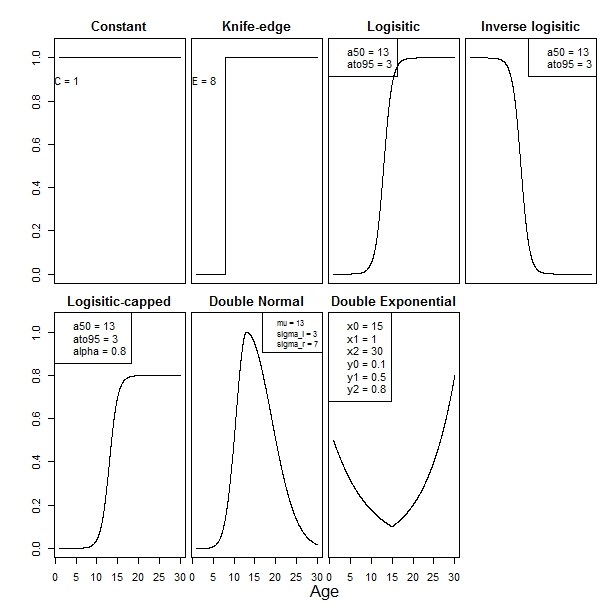
\includegraphics[scale = 0.7]{Figures/Selectivities.jpeg}
	\caption{Examples of the functional forms of selectivities available in \CNAME.}
\end{figure}

Selectivities \subcommand{all\_values} and \subcommand{all\_values\_bounded} can be addressed in additional priors using the following syntax,

{\small{\begin{verbatim}
		@selectivity maturity
		type all_values
		v 0.001 0.1 0.2 0.3 0.4 0.3 0.2 0.1

		## encourage ages 3-8 to be smooth.
		@additional_prior smooth_maturity
		type vector_smooth
		parameter selectivity[maturity].values{3:8}

		\end{verbatim}}}

\subsection{\I{Projections}\label{sec:projections}}

This section lists all the projections classes available, their functionality and an example of the syntax.

\subsubsection[Constant]{\argument{constant}}\index{Projections!Constant}

A parameter can either be fixed during all projection years or specified individually for each projection year. This is a deterministic assumption, where the parameter is assumed to be known without error during projection years.

{\small{\begin{verbatim}
		@project Future_ycs
		type constant
		parameter process[Recruitment].ycs_values
		years 2012:2016
		values 1 2 1 2 0.5
		multiplier 1
		\end{verbatim}}}

\subsubsection[Empirical resampling]{\argument{empirical\_resampling}}\index{Projections!Empirical resampling}

Parameters that have time components associated with them can be re-sampled uniformly with replacement over a range of years and used as the projected years' values. The year range which users must specify are between \argument{start\_year} and \argument{final\_year}
{\small{\begin{verbatim}
		@project Future_ycs
		type empirical_sampling
		parameter process[Recruitment].ycs_values
		years 2012:2016
		start_year 1988
		final_year 2008
		multiplier 1
		\end{verbatim}}}


\subsubsection[Lognormal]{\argument{lognomral}}\index{Projections!Lognormal}

The parameters are originally drawn from a Gaussian distribution in log space and exponentiated out to form the lognormal distribution,

\begin{equation}\label{eq:lognormal}
X_p = e^{\epsilon_p- 0.5\sigma^2}
\end{equation}

where $\epsilon_p\stackrel{iid}{\sim}N(\mu,\sigma)$ and $X_p$ is the projected value for parameter $X$, and $\mu$, $\sigma$ is the mean and standard deviation on the log scale. An example of applying this process is if we wanted to draw future year class parameters from a lognormal distribution with mean 1 and standard deviation 0.8, we would define the syntax as,

{\small{\begin{verbatim}
		@project Future_ycs
		type lognormal
		parameter process[Recruitment].ycs_values
		years 2012:2016
		mean 0
		sigma 0.8
		multiplier 1
		\end{verbatim}}}

\subsubsection[Lognormal-Empirical]{\argument{lognomral\_empirical}}\index{Projections!Lognormal-Empirical}

This class applies a lognormal draw as in the \argument{LogNormal} class but it allows the user to specify a year range which is re-sampled uniformly without replacement. These re-sampled values are then used to calculate the standard deviation of the distribution. Then equation~\eqref{eq:lognormal} is used to generate future values with user defined $\mu$ and empirically calculated $\sigma$,

{\small{\begin{verbatim}
		@project Future_ycs
		type lognormal_empirical
		parameter process[Recruitment].ycs_values
		years 2012:2016
		mean 0
		start_year 1988
		final_year 2008
		multiplier 1
		\end{verbatim}}}

\subsubsection[User Defined]{\argument{user\_defined}}\index{Projections!User Defined}

This class allows the use of the equation parser to define the future values of a parameter during projection mode. This was originally set-up to apply harvest control rules (i.e. apply a management action such as changing the TACC based on the current or previous state). In fisheries, this would be setting the catch based on an exploitation rate multiplied by the vulnerable biomass, where the exploitation rate is based on some rule as shown in figure~\ref{fig:HCR}.

\begin{figure}[!h]
	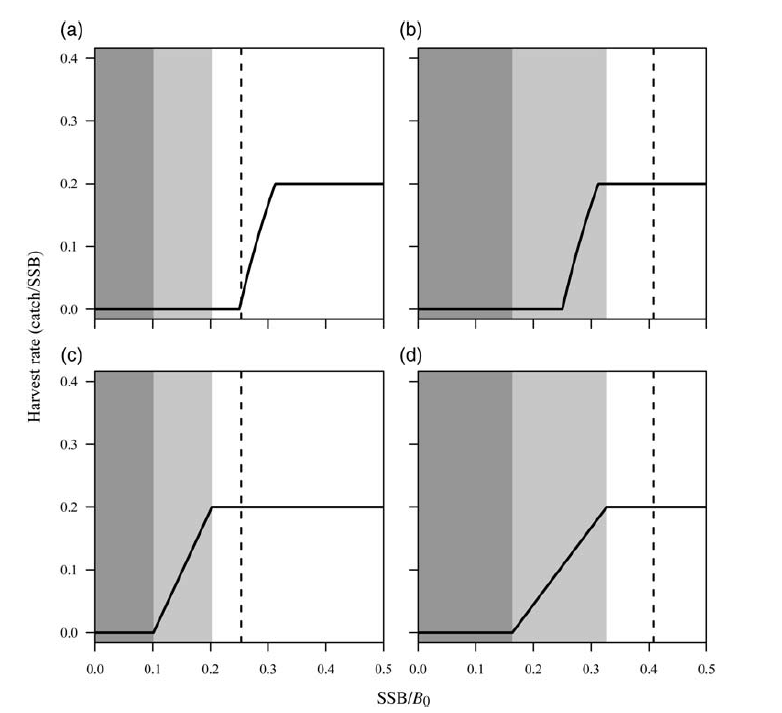
\includegraphics[scale=0.9]{Figures/HarvestControlRules.png}
	\caption{\textbf{Examples of control rules based on current stock status.}}
	\label{fig:HCR}
\end{figure}

\pagebreak
{\small{\begin{verbatim}
		@project HCR_2015
		type user_defined
		parameter process[Instantaneous_Mortality].method_Sub_Ant_F
		years 2015
		equation if(derived_quantity[SSB].values{2014} / process[Recruitment].b0 <= 0.1, 0.0,
		if(derived_quantity[SSB].values{2014} / process[Recruitment].b0 > 0.1 &&
		derived_quantity[SSB].values{2014} / process[Recruitment].b0 < 0.2,
		derived_quantity[SSB].values{2014} * derived_quantity[SSB].values{2014}
		/ process[Recruitment].b0,
		derived_quantity[SSB].values{2014} * 0.2))
		\end{verbatim}}}

The syntax of the equation parser can be messy and care should be taken when writing it. In words the above equation is, if $\%B_{2014} \leq 0.1$ then set next years catch to 0.0, else if $\%B_{2014} > 0.1 \text{ } \& \text{ } \%B_{2014} \leq 0.2$ then set next years catch equal to $\%B_{2014} \times SSB_{2014}$, else set next years catch to $0.2 SSB_{2014}$.

\subsubsection[Catches]\index{Projections!Catches}
Catches are unique in that they are known inputs in a table format. To project catches that are in a table use this example projection block,
{\small{\begin{verbatim}
# fishing process
@process Fishing
type mortality_instantaneous_retained
m 0.17*6  #0.17    #testing at old values
time_step_ratio 1
selectivities One*6   #for age based M
categories *
table catches
year	FishingLine	FishingPot	Recreation
1900	0	0	0
1901	13.2	0	22.9
1902	26.4	0	23.5
1903	39.6	0	24
end_table

# projection block
@project future_catch
type constant
parameter process[Fishing].method_fishingpot
years 2020:2029
values 4000
\end{verbatim}}}

This follows the syntax, \texttt{block\_type[block\_label].method\_fishinglabel}. \textbf{note} the fishing label which is defined in the table needs to be lower case form in the \command{projection} block.

\subsection{\I{Time Varying Parameters}\label{sec:time_var}}

\CNAME\ has the functionality to vary any parameter annually between the start and final year of a model run. This can be for blocks of years or specific years. For years that are not specified the parameter will default to the input, or if in an iterative state such as estimation mode, the value being trialled at that iteration. Method types for time varying a parameter are; \subcommand{constant}, \subcommand{random\_walk}, \subcommand{exogenous}, \subcommand{linear}, \subcommand{annual\_shift}, \subcommand{random\_draw}. This allows users to let a parameter be known in a year, be the result of a deterministic equation, or stochastic. \textbf{Note} stochastic time varying was added for simulation purposes. It has not been tested in an estimation context. To implement hierarchical I have estimated the prior values with hyper-priors. If you were to try an implement a hierarchical model using the time varying functionality, firstly you could only do this at MCMC estimation because an MPD we would not be doing that integral which is required to obtain unbiased estimates. In an MCMC context you would be assuming a Gibbs sampler. That is every draw is from a conditional distribution and so every draw is a candidate value.

When allowing removals to have annual varying catchabilities, selectivities and other more realistic model components, simulated observations more closely model real data and associated conclusions become more useful. Another driver for implementing time-varying parameters was allowing mean or location parameters of selectivities to change between years based on an explanatory variable. An example of this is in the New Zealand Hoki fishery where we allow the $\mu$ and $a_{50}$ parameters to shift depending on when the fishing season occurs. Descriptive analysis showed that when fishing was earlier relative to other years smaller fish were caught and vice versa. This can be shown in the CASAL2/Examples/2stock directory, implemented at line: \texttt{382} in the \texttt{population.csl2} file.

\subsubsection[Constant]{\argument{constant}}\index{Time Varying Parameters!Constant}
Allows a parameter to have an alternative value during certain years, which can be estimated.
{\small{\begin{verbatim}
		@time_varying q_time_var
		type constant
		parameter catchability[survey_q].q
		years 1975:1988
		values 0.001
		\end{verbatim}}}

Users can also estimate these year values using the following syntax, caution is that you shouldn't estimate the actual parameter and its time varying counterpart, as the time varying value will overwrite the actual parameter making the first value unidentifiable and an impossible optimization process.
{\small{\begin{verbatim}
		@estimate q_time_var
		type uniform
		parameter time_varying[q_time_var].values(1975:1976)
		lower_bound 1e-6 1e-6
		upper_bound 2 2
		\end{verbatim}}}

\textbf{Caution required}: the actual parameter and its time varying counterpart should not both be estimated, as the time varying value will overwrite the actual parameter making the first value unidentifiable and an impossible optimization process.

\subsubsection[Random Walk]{\argument{random\_walk}}\index{Time Varying Parameters!Random Walk}

A random deviate is added into the last value drawn from a standard normal distribution. This has an estimable parameter $\sigma_p$ for each time varying parameter $p$. For reproducible modelling, it is highly recommended that users set the seed (see Section~\ref{sec:command-line-arguments}) when using stochastic functionality like this, otherwise reproducing models becomes almost impossible.
{\small{\begin{verbatim}
		@time_varying q_time_var
		type random_walk
		parameter catchability[survey_q].q
		distribution normal
		mean 0
		sigma 3
		\end{verbatim}}}

If the \texttt{parameter} specified in the \command{time\_varying} block is associated with an \command{estimate} block then the parameter is constrained to stay within the lower and upper bounds of the \command{estimate} block. \textbf{WARNING}, if the parameter does not have an associated \command{estimate} block then there is no safe guard for a random deviate to put the parameter in a space where the model fails, i.e generates NA or INF values. To avoid this, we recommended an \command{estimate} block is specified even though the parameter is not actually being estimated, see example syntax, below. A constraint whilst using this functionality is that a parameter cannot be less than 0.0, if it is \CNAME\ sets it equal to 0.01.

{\small{\begin{verbatim}
		@estimate survey_q_est
		type uniform
		parameter catchability[survey_q].q
		lower_bound 1e-6
		upper_bound 10
		\end{verbatim}}}
This will insure the random walk time varying process will set the any new candidate within the lower and upper bound of the \command{estimate} block.

\subsubsection[Annual shift]{\argument{annual\_shift}}\index{Time Varying Parameters!Annual shift}

A parameter generated in year $y$ ($\theta'_y$) depends on the value specified by the user ($\theta_y$) along with three coefficients $a,b$ and $c$ as follows,

\begin{equation}
\bar{\theta}_y = \frac{\sum_{y}^Y\theta_y}{Y}
\end{equation}

\begin{equation}
\theta'_y = a \bar{\theta}_y + b\bar{\theta}_y^{2} + c\bar{\theta}_y^{3}
\end{equation}

\subsubsection[Exogenous]{\argument{exogenous}}\index{Time Varying Parameters!Exogenous}

Parameters are shifted based on an exogenous variable, an example of this is an exploitation selectivity parameters that may vary between years based on known changes in exploitation behaviour such as season, start time, and average depth of exploitation.

\begin{equation}
\delta_y = a(E_y - \bar{E})
\end{equation}

\begin{equation}
\theta'_y = \theta_y + \delta_y
\end{equation}

where $\delta_y$ is the shift or deviation in parameter $\theta_y$ in year $y$ to generate the new parameter value in year $y$ ($\theta'_y$). $a$ is an estimable shift parameter, $E$ is the exogenous variable and $E_y$ is the value of this variable in year $y$. For more information readers can see \cite{francis_03}.

\subsection{\I{Equation Parser}\label{sec:eq_parser}}

\CNAME\ has the ability to use an equation parser, this is currently implemented in Projections (section~\ref{sec:projections}), Derived quantities (section~\ref{sec:derived-quantities}) and Reports (section~\ref{sec:report-section}). Examples of syntax for implementing the equation parser follow from here. For a more detailed look at the parser see \url{https://github.com/nickgammon/parser/blob/master/parser.cpp}\\


{\small{\begin{verbatim}
		equation process[Recruitment].r0 * (2-1)
		\end{verbatim}}}

and can apply routine mathematical functions such as \texttt{log},  \texttt{exp},  \texttt{cos}, \texttt{sin}, \texttt{tan}, e.g.,
{\small{\begin{verbatim}
		equation sqrt(process[Recruitment].r0)
		\end{verbatim}}}

apply exponents,
{\small{\begin{verbatim}
		equation pow(2, 3)
		\end{verbatim}}}

evaluate the absolute of an equation using the \texttt{abs()} syntax,
{\small{\begin{verbatim}
		equation abs(sqrt(process[Recruitment].r0) * 1.33)
		\end{verbatim}}}

use if else statements
{\small{\begin{verbatim}
		equation if(process[Recruitment].r0 > 23, 44, 55)
		## if R0 is greater than 23 return 44 else return 55
		\end{verbatim}}}

if else statements can also be linked, but the syntax becomes a little messy, e.g.,
{\small{\begin{verbatim}
		equation if(process[Recruitment].r0 > 23, 44,
         		if(process[Recruitment].r0 > 10, 55, 66))
		## if R0 is greater than 23 return 44 else if R0 less than 23 but greater than 10 return 55,
		else R0 must be less than 10 return 66
		\end{verbatim}}}

Only singletons can be reference, so an equation cannot be applied to vector parameters, e.g. \subcommand{process[Recruit].ycs\_values\{1974:1980\}} can't be referenced. To see which parameters can be included in an equation parser go to the syntax section (Section~\ref{sec:syntax}). Any subcommand that has a \texttt{type estimable} could, in theory, be addressed in an equation parser.

With the equation parser it is difficult to catch all user configuration errors, we cannot check whether a parameter that exists in the system has been populated when the user requires it. For example, the wrong year could easily be misspecified in the case of next years (2015) removals to be based on the this years (2014) state of the population,
{\small{\begin{verbatim}
		parameter process[removals].catch
		year 2015
		equation derived_quantity[percent_b0].values{2020}
		\end{verbatim}}}

The above would be an acceptable equation but obviously will cause nonsensical results, because you are asking for a value in 2020 when you are in 2015. This is just a caution, for although the equation parser adds a great deal of flexibility, users should be careful because it is easy to misspecify models in this manner.
